\documentclass[journal]{IEEEtran}

\usepackage[T1]{fontenc}

\usepackage{cite}
\usepackage{amsmath}
\interdisplaylinepenalty=2500
\usepackage{amssymb}
\usepackage{amsthm}
\usepackage{graphicx}
\usepackage{booktabs}
\usepackage{array}
\usepackage[caption=false,font=footnotesize,labelformat=simple,justification=centering]{subfig}
\usepackage{url}
\usepackage[hidelinks]{hyperref}
% URLs break only after a slash or a dot, never right after "https:" (":" is a relation by default, and the
% url package prefers a break there); as an "open" character it allows no break.
\def\UrlBigBreaks{}
\def\UrlBreaks{\do\/\do\.\do\-\do\_}
\def\UrlNoBreaks{\do\(\do\[\do\{\do\<\do\:}

% Shared notation for every section (do not redefine elsewhere)
\newcommand{\BIG}{\mathsf{B}}                       % value of a passed pawn, B = 256
\newcommand{\pos}[1]{\texttt{#1}}                   % pawn list, e.g. \pos{W a2 c2 / B b7 d7}
\newcommand{\fen}[1]{\texttt{\small #1}}
\newcommand{\lab}[1]{\textsf{\footnotesize[#1]}}   % evidence label: \lab{P}, \lab{S}, \lab{C2}, \lab{C1}, \lab{Conj}
\newcommand{\nim}[1]{\mathord{\star#1}}             % nimbers, as in the 2025 paper: \star, \nim{2}
\newcommand{\upsec}{\mathord{\uparrow^{2}}}         % up-second {0 | down star}
\newcommand{\tinyg}[1]{\operatorname{tiny}(#1)}
\newcommand{\game}[2]{\{\,#1 \mid #2\,\}}
\newcommand{\ggame}[2]{\{\,#1 \parallel #2\,\}}
\newcommand{\cyl}[1]{C_{#1}}                        % n-file cylinder
\newcommand{\flatb}[1]{F_{#1}}                      % n-file flat board
\newcommand{\repourl}{https://github.com/aritroBh/cylindrical-chess-cgt}


% Two builds. main.tex is the named (arXiv) build. main_review.tex defines \anonbuild and inputs this file,
% which gives the double-anonymous review build for IEEE Transactions on Games.
% \submittedtrue adds IEEE's preprint notice to the named build. Turn it on only once the paper has been
% submitted to the IEEE (GUIDELINES F); it never appears in the review build.
\newif\ifsubmitted
\submittedfalse
\ifdefined\anonbuild
  \newcommand{\codeurl}{}
  \newcommand{\codeavail}{available in an anonymized repository supplied to the editor}
  \newcommand{\bytheauthor}{}
  \newcommand{\studyauthor}{Anonymous}
  \newcommand{\studytitle}{Title withheld for review}
  \hypersetup{pdftitle={Chess Endgames on a Cylindrical Chessboard: Exact Combinatorial Game Values,
    Real-Chess Checks, and Tablebases}, pdfauthor={}}
\else
  \newcommand{\codeurl}{\url{https://github.com/aritroBh/cylindrical-chess-cgt}}
  \newcommand{\codeavail}{available at \codeurl}
  \newcommand{\bytheauthor}{ by the author}
  \newcommand{\studyauthor}{A.~Bhattacharjee}
  \newcommand{\studytitle}{Analysis of chess endgames on a cylindrical chessboard}
  \hypersetup{pdftitle={Chess Endgames on a Cylindrical Chessboard: Exact Combinatorial Game Values,
    Real-Chess Checks, and Tablebases}, pdfauthor={Aritro Bhattacharjee}}
\fi

% The sections use the subcaption-style environment
%   \begin{subfigure}[pos]{width} ... \caption{...}\label{...} \end{subfigure}.
% IEEEtran's captions are kept by implementing it with subfig's \subfloat (caption=false), as the
% IEEEtran HOWTO recommends. A subfigure is labelled (a) and referenced as Fig. 3(a).
\renewcommand{\thesubfigure}{(\alph{subfigure})}
\makeatletter
\newsavebox{\sf@box}
\newcommand{\sf@setcap}[2][]{\gdef\sf@cap{#2}}
\newcommand{\sf@setlab}[1]{\gdef\sf@lab{#1}}
\newenvironment{subfigure}[2][c]{%
  \gdef\sf@cap{}\gdef\sf@lab{}%
  \begin{lrbox}{\sf@box}\begin{minipage}[#1]{#2}%
  \let\caption\sf@setcap\let\label\sf@setlab}%
  {\end{minipage}\end{lrbox}%
   \ifx\sf@lab\@empty\def\sf@labcmd{}\else\edef\sf@labcmd{\noexpand\label{\sf@lab}}\fi
   \ifx\sf@cap\@empty\subfloat[]{\usebox{\sf@box}\sf@labcmd}%
   \else\subfloat[\sf@cap\sf@labcmd]{\usebox{\sf@box}}\fi}
\makeatother

% One counter for all numbered statements, through the whole paper, in IEEE style:
% an indented italic head ending in a colon ("Theorem 2 (Cut lemma; [P]):"). A head whose note is
% only an evidence label prints it without parentheses ("Proposition 4 [P]:").
\makeatletter
\def\ieeethmnote#1{\ieee@thmnote#1\@empty\@nil}
\def\ieee@thmnote#1#2\@nil{\ifx#1\lab\expandafter\@firstoftwo\else\expandafter\@secondoftwo\fi
  {\lab#2}{(#1#2)}}
\makeatother
\newtheoremstyle{ieeeplain}{3pt}{3pt}{\itshape}{\parindent}{\itshape}{:}{0.5em}%
  {\thmname{#1}\thmnumber{ #2}\thmnote{ \ieeethmnote{#3}}}
\newtheoremstyle{ieeedef}{3pt}{3pt}{\normalfont}{\parindent}{\itshape}{:}{0.5em}%
  {\thmname{#1}\thmnumber{ #2}\thmnote{ \ieeethmnote{#3}}}
\theoremstyle{ieeeplain}
\newtheorem{theorem}{Theorem}
\newtheorem{lemma}[theorem]{Lemma}
\newtheorem{proposition}[theorem]{Proposition}
\newtheorem{corollary}[theorem]{Corollary}
\newtheorem{conjecture}[theorem]{Conjecture}
\theoremstyle{ieeedef}
\newtheorem{definition}[theorem]{Definition}
\newtheorem{remark}[theorem]{Remark}
% Proofs use IEEEtran's proof layout; \begin{proof}[Proof sketch] prints "Proof sketch:".
\renewenvironment{proof}[1][Proof]{\begin{IEEEproof}[#1]}{\end{IEEEproof}}

\hyphenation{tr\'e-bu-chet tr\'e-bu-chets table-base table-bases}

\begin{document}

\title{Chess Endgames on a Cylindrical Chessboard: Exact Combinatorial Game Values, Real-Chess Checks,
and Tablebases}

\ifdefined\anonbuild
\author{Anonymized for review}
\markboth{IEEE Transactions on Games}{Chess Endgames on a Cylindrical Chessboard}
\else
\ifsubmitted
  \newcommand{\ieeenotice}{\thanks{This work has been submitted to the IEEE for possible publication.
    Copyright may be transferred without notice, after which this version may no longer be accessible.}}
\else
  \newcommand{\ieeenotice}{}
\fi
\author{Aritro~Bhattacharjee%
\ieeenotice
\thanks{A.~Bhattacharjee, e-mail: aritro.sonu@gmail.com.}}
\markboth{Bhattacharjee: Chess Endgames on a Cylindrical Chessboard}%
{Bhattacharjee: Chess Endgames on a Cylindrical Chessboard}
\fi

\maketitle

\begin{abstract}
Cylinder chess joins the a-file to the h-file, so the board has no edges or corners. We study its
king-and-pawn endgames with combinatorial game theory, following Elkies: a passed pawn wins, and the kings are
frozen in a mutual zugzwang worth zero. We repair this model with a passed-pawn test that respects en
passant, and give conditions under which the frozen kings are exact. Under the new
test, an exhaustive census finds no nimber above star with at most six pawns on ordinary boards up to four
files wide, but star two appears with seven, in one position and its color-reversed twin, confirmed by three
programs; on the three-file cylinder six pawns suffice. We also find king-and-pawn positions worth
one-eighth, up-second star and Tiny 1, and test them against real chess: with frozen kings and queen
promotions only, the one-eighth hinges on one side of one end position. Four-man tablebases on the cylinder
and the torus confirm that king and rook can no longer force mate; on the cylinder, opposite-colored bishops
still can. We correct earlier work on cylinder Dawson's
chess: the full ring is a first-player win exactly when the strip three files shorter has Grundy value
zero.
\end{abstract}

\begin{IEEEkeywords}
Chess, combinatorial game theory, endgame tablebases, game solving, nimbers.
\end{IEEEkeywords}


% Table of contents: named (arXiv) build only; the author asked for one. The review build omits it.
\ifdefined\anonbuild\else
\begingroup
\makeatletter
\footnotesize
\setcounter{tocdepth}{1}
\renewcommand{\l@section}[2]{\par\noindent\hangindent 2.4em #1\nobreak\hfill #2\par}
\renewcommand{\numberline}[1]{\makebox[2.4em][l]{#1}}
\section*{\contentsname}
\vspace{-0.4\baselineskip}
\@starttoc{toc}
\makeatother
\endgroup
\vspace{0.3\baselineskip}
\fi

\section{Introduction}\label{sec:intro}

\IEEEPARstart{C}{ylinder} chess is ordinary chess on a board whose a-file and h-file are joined
\cite{Pritchard}: a white pawn on h4 can capture on a5, a king on a1 can step to h2, and there are no side edges or
corners. We use combinatorial game theory (CGT) to study its king-and-pawn endgames.

Under normal play the player who cannot move loses; CGT gives each position a value, and a sum of independent
games has the sum of their values \cite{ONAG,WinningWays,Siegel2013}. Chess can be drawn and its kings roam,
yet Elkies \cite{Elkies1996} showed that many pawn endgames split into local fights with exact values, under
two conventions:
\begin{itemize}
\item a passed pawn wins, and is worth a large number $\pm\BIG$;
\item the kings stand in a mutual zugzwang, the \emph{tr\'ebuchet}, worth $0$.
\end{itemize}

The cylinder changes this picture in three ways. There are no rook pawns, and shifting a position sideways
does not change its value. A position with a pawn on every file, a \emph{ring}, has no edge at which to cut
it. And the corners that decide mates and fortresses are gone.

A nimber $\nim{k}$ is a game in which either player may move to any of $\nim{0}=0$, $\nim{1}=\star$,
\dots, $\nim{(k-1)}$. The simplest after $\star=\game{0}{0}$ is $\nim{2}=\game{0,\star}{0,\star}$: either player
may move to $0$ or to $\star$. Elkies built higher nimbers on large boards from Dawson's pawn game \cite{Elkies2002,Dawson1935}, and
Drummond-Cole built positions of value $\nim{2}$ in chess with the help of pieces other than kings and
pawns~\cite{DrummondCole2005}. We ask whether $\nim{2}$ occurs in a king-and-pawn endgame on an 8-rank board,
the \emph{$\nim{2}$ question}, and whether real chess agrees.

This paper extends an unpublished 2025 study of the basic values\bytheauthor~\cite{Study2025}: we check
every position by computer, correct its errors and carry the analysis on, in the position-by-position format
of Wu, Y\"u and Landry~\cite{WuYuLandry2010}. Theorems and headline numbers
carry labels: \lab{P}, proved here; \lab{AI}, proof given or sketched here (in full in the
repository), checked by AI models, human check pending; \lab{C2}, two independently written programs agree,
the second written from the rules alone; \lab{C1}, one program; \lab{Conj}, a conjecture. Our contributions
are:
\begin{itemize}
\item \emph{Model} (Sections~\ref{sec:rules} and~\ref{sec:sums}): a passed-pawn test that respects en passant,
  a cut lemma \lab{P}, a sum-safety theorem \lab{AI}, and a position showing that checking only the
  top-level components is not enough \lab{C2}.
\item \emph{Kings} (Section~\ref{sec:kings}): conditions (V1)--(V3) under which a frozen tr\'ebuchet gives the
  result of the whole-board pawn game \lab{AI}, and (V4) for the $\pm\BIG$ value \lab{AI}.
\item \emph{Small values} (Sections~\ref{sec:basic}, \ref{sec:atlas} and~\ref{sec:targets}): cylinder-only values
  come from rings \lab{P}; $1/8$ and $\upsec\star$ \lab{C2}, and Tiny~1 \lab{C1}, occur in 10-man positions
  with a legal pawn history.
\item \emph{The $\nim{2}$ question} (Section~\ref{sec:star2}): in the default setting (count rule, e.p.-aware
  test; Section~\ref{sec:ep}) no $\nim{2}$ has six
  pawns or fewer on ordinary boards of any width, but $\nim{2}$ appears with seven
  \lab{C2}; on the cylinder $\cyl{3}$ a six-pawn ring suffices \lab{C2}, as a whole-board game some ring with $n+3$
  pawns is $\nim{2}$ on every $\cyl{n}$ with $n\ge5$ \lab{AI}, and on $\cyl{7}$ some ten-pawn rings are
  $\nim{3}$ \lab{C2}.
\item \emph{Real chess} (Section~\ref{sec:real}): with the new test the textbook $\nim{2}$ candidate is not
  $\nim{2}$, however draws are treated; with queen promotions only and frozen kings, the oracle value of the $1/8$ position
  is exactly $1/8$ \lab{C1}.
\item \emph{Tablebases} (Section~\ref{sec:tb}): king and rook win only 2.80\% of cylinder positions, and on the
  torus only two major pieces force mate \lab{C2}.
\item \emph{Dawson's chess} (Section~\ref{sec:dawson}): the $3\times n$ cylinder is a first-player win if and
  only if the $3\times(n-3)$ strip has Grundy value $0$ \lab{P}.
\item \emph{Engines} (Section~\ref{sec:engines}): Stockfish is weakest on infinitesimals at low depth, and on sums
  of components engines often miss the model's winning moves \lab{C1}.
\end{itemize}

Sections~\ref{sec:rules} and~\ref{sec:basic} set up the rules and the basic values,
Sections~\ref{sec:kings} and~\ref{sec:sums} add kings and sums, Sections~\ref{sec:atlas}--\ref{sec:star2}
search for small values and $\nim{2}$, and Section~\ref{sec:real} tests them against real chess.
Sections~\ref{sec:tb}--\ref{sec:engines} turn to tablebases, Dawson's chess and engines,
Section~\ref{sec:verify} gives the cross-checks and the code, Section~\ref{sec:conclusion} lists open
problems, and the Appendix gives the FEN of each position with kings.

\section{Rules, Values and Conventions}\label{sec:rules}

\subsection{The Board and the Moves}
We play ordinary chess on the \emph{cylinder}, the $8\times8$ board with the a-file joined to the h-file. Only
the files wrap: ranks 1 and 8 are still edges. Every piece may cross the seam: a white pawn on h4 can capture on
a5, a knight on h1 gains a3 and b2, and a king on h1 gains a1 and a2, so a checkmate on the ordinary board need
not be one on the cylinder. A sliding piece stops before its ray returns to its own square, so a rook cannot
circle a rank as a null move. En passant (e.p.) is allowed, across the seam too. We write $\cyl{n}$ and
$\flatb{n}$ for the cylinder and the ordinary board with $n$ files and eight ranks.

\subsection{Notation}\label{sec:notation}
We write $G=\game{G^L}{G^R}$ when white (Left) can move to the positions $G^L$ and black (Right) to $G^R$, and
$G+H$ for the sum in which the player to move chooses one component~\cite{WinningWays,ONAG,Siegel2013}. Every
finite game has a unique \emph{canonical form}, obtained by deleting dominated options and bypassing reversible
ones, and $G=H$ exactly when $G-H$ is a second-player win. The \emph{outcome class} of $G$ is $\mathcal{L}$ if
white wins whoever starts, $\mathcal{R}$ if black does, $\mathcal{N}$ if the first player wins and
$\mathcal{P}$ if the second does. Our values include \emph{numbers} (integers and dyadic fractions such as
$1/2=\game{0}{1}$), \emph{nimbers} $\nim{k}$ (Section~\ref{sec:intro}), and \emph{switches} $\pm x=\game{x}{-x}$ with $x>0$. Sums are written without the plus sign,
so for a number $a$, $a\pm x=a+(\pm x)=\game{a+x}{a-x}$. The \emph{birthday} of a game is the height of its
canonical game tree, so $\nim{k}$ has birthday $k$. Each game has a \emph{mean} and a \emph{temperature}, read
from its thermograph~\cite{WinningWays}; $\pm x$ has mean $0$ and temperature $x$. The \emph{left} and
\emph{right stops} of $G$ are the numbers reached when white or black moves first and both sides play until a
number appears; both stops of $0$ and of $\nim{2}$ are $0$. Infinitesimals such as ${\uparrow}=\game{0}{\star}$ and
$\tinyg{1}=\ggame{0}{0\mid -1}$ are introduced with their positions in Section~\ref{sec:basic}.

\subsection{Normal Play and the Passed-Pawn Convention}
Following Elkies~\cite{Elkies1996}, we change chess just enough to fit normal play~\cite{WinningWays}.
\begin{itemize}
\item In pawn-only positions, a player who has no move loses; there are no null moves.
\item A position in which exactly one side has a passed pawn is decided, worth $+\BIG$ if that pawn is white and
  $-\BIG$ if it is black, where $\BIG$ exceeds any count of spare moves (our programs use $\BIG=256$).
\item Kings are added as a group in mutual zugzwang, the tr\'ebuchet, and are then \emph{frozen}: the model
  never moves them and counts the group as $0$, since whoever moves a king there first loses a pawn, and then
  the game. Section~\ref{sec:kings} asks when this is exact.
\end{itemize}
A move, usually a capture, can give both sides a passed pawn; such a race needs a rule:
\begin{itemize}
\item \emph{count}: fewer moves to promote wins; the side that did not move goes first and wins a tie;
\item \emph{mover}: the side that made the move wins;
\item \emph{opponent}: the other side wins.
\end{itemize}
None is exact chess, since a new queen may give check or stop the other pawn.

\subsection{En Passant and the Passed-Pawn Test}\label{sec:ep}
The textbook test calls a pawn passed if no enemy pawn stands ahead of it on its own file or a neighboring file
(on the cylinder, a and h are neighbors). En passant breaks this test: after a2--a4 in Fig.~\ref{fig:ep_test}
the textbook test calls the a-pawn passed, yet black takes it en passant, b4$\times$a3. Elkies asked for a
more systematic treatment of en passant~\cite{Elkies1996}; we use a stricter test.

\begin{figure}[!t]
\centering
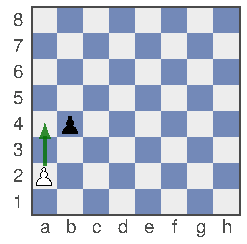
\includegraphics[width=0.36\columnwidth]{figures/ep_test.pdf}
\caption{Position \pos{W a2 / B b4} (ordinary board), value $0$. After a2--a4 (arrow) the textbook test calls the
a-pawn passed, but b4$\times$a3 en passant removes it; under Definition~\ref{def:epaware} it is not passed.}
\label{fig:ep_test}
\end{figure}

% Fig. 2 belongs to Section III; it is defined here so that the full-width float lands next to it.
\begin{figure*}[!t]
\centering
\begin{subfigure}[t]{0.16\textwidth}\centering
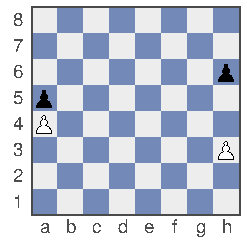
\includegraphics[width=\linewidth]{figures/zero_seam.pdf}
\caption{\pos{W~a4~h3 / B~a5~h6}: $0$}
\end{subfigure}\hfill
\begin{subfigure}[t]{0.16\textwidth}\centering
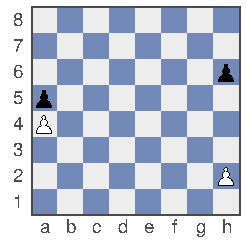
\includegraphics[width=\linewidth]{figures/one.pdf}
\caption{\pos{W~a4~h2 / B~a5~h6}: $1$}
\end{subfigure}\hfill
\begin{subfigure}[t]{0.16\textwidth}\centering
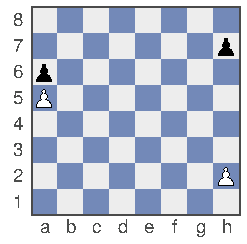
\includegraphics[width=\linewidth]{figures/two.pdf}
\caption{\pos{W~a5~h2 / B~a6~h7}: $2$}
\end{subfigure}\hfill
\begin{subfigure}[t]{0.16\textwidth}\centering
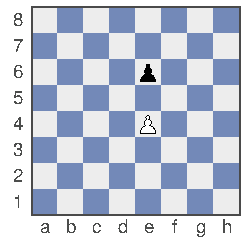
\includegraphics[width=\linewidth]{figures/star.pdf}
\caption{\pos{W~e4 / B~e6}: $\star$}
\end{subfigure}\hfill
\begin{subfigure}[t]{0.16\textwidth}\centering
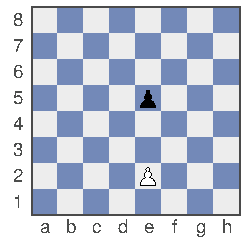
\includegraphics[width=\linewidth]{figures/up.pdf}
\caption{\pos{W~e2 / B~e5}: ${\uparrow}$}
\end{subfigure}\hfill
\begin{subfigure}[t]{0.16\textwidth}\centering
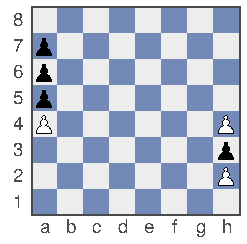
\includegraphics[width=\linewidth]{figures/tiny1_2025.pdf}
\caption{\pos{W~a4~h2~h4 / B~a5~a6~a7~h3}: $\tinyg{1}$}
\end{subfigure}
\caption{Pawn positions with the basic values (cylinder: files a and h adjacent). Each value holds in all nine
settings (Section~\ref{sec:ep}) except in (c), which is $2$ only with e.p.\ on and ${\Uparrow}\star$ with
e.p.\ off.}
\label{fig:basic}
\end{figure*}

\begin{definition}[E.p.-aware passed pawn]\label{def:epaware}
A pawn is \emph{passed} if it passes the textbook test \emph{and} cannot be captured en passant on the
opponent's next move.
\end{definition}

One more white pawn makes the difference decisive. In \pos{W~a2~b3 / B~b4} black has no move, and the textbook
test lets white win at once with a2--a4. Under Definition~\ref{def:epaware}, every white move lets black capture
on a3, directly or en passant, and win the race that follows under the count rule, so the value is $0$. Across
the census of Section~\ref{sec:atlas}, every position with at most six pawns on ordinary boards of width at
most four, the stricter test changes at least $18{,}137$ of the $231{,}071$ values (a few more changes are hidden
where both values exceed the display range), and $4{,}070$ of them in outcome \lab{C1}.

The three race rules and three e.p.\ options (textbook test, e.p.-aware test, e.p.\ off) give nine
\emph{settings}. Every value uses the \emph{default setting}, the count rule with the e.p.-aware test, unless
we say otherwise.

\subsection{Components and the Cut Lemma}
A pawn changes file only by capturing onto a file where an enemy pawn stands (en passant included), so an empty
file stays empty forever and the pawns on either side of it never interact. Each block of neighboring occupied
files is a game of its own, a \emph{component}, and a position is the sum of its components; on the cylinder a
component is an arc or one \emph{ring} that uses every file.

\begin{theorem}[Cut lemma; \lab{P}, \lab{C2}]\label{thm:cut}
A pawn position on $\cyl{n}$ with at least one empty file has the same value as the position on
$\flatb{n-1}$ obtained by cutting the cylinder open along that file.
\end{theorem}

\begin{proof}
No pawn can move onto the empty file, so cutting the board there changes no legal move, no en passant right and
no passed-pawn test: the files beside the cut lose only a neighbor that stays empty forever.
\end{proof}

Hence values only a cylinder can make must come from rings (Section~\ref{sec:atlas});
Section~\ref{sec:sums-hss} says when a sum of components still names the right winner.

\section{Basic Positions on the Cylinder}\label{sec:basic}

We now build the basic values of Fig.~\ref{fig:basic} with pawns alone. Each board leaves a file empty, so by
Theorem~\ref{thm:cut} its value is that of an ordinary-board position, cut open along that
file~\cite{Elkies1996,WuYuLandry2010}; in four of them the play crosses the seam. A move that the
opponent can answer with a passed pawn is a losing move, and it drops out, since having only losing moves is
the same as having no moves at all~\cite{WuYuLandry2010}. A move that the opponent can answer by reaching a
position at least as good for him as the one we started from is \emph{reversible}: in the canonical
form~\cite{WinningWays} it is replaced by the player's moves from that reply, and so drops out when there are
none.

\subsection{The Zero Game}
Let us begin with the zero game, in which neither player can move: $0=\game{}{}$, a second-player win. In
\pos{W~e4 / B~e5} the two pawns are stuck, so the value is $0$.

Fig.~\ref{fig:basic}(a) is a zero game that uses the seam. If white goes first, it must play h3--h4, and black
captures across the seam, a5$\times$h4, with a passed pawn. If black goes first, h6--h5 is met by a4$\times$h5.
Whoever moves first loses: again $0$.

\subsection{The Games \texorpdfstring{$1$}{1} and \texorpdfstring{$2$}{2}}
In Fig.~\ref{fig:basic}(b) the white h-pawn starts one square further back. White can play h2--h3, which leaves
the zero game of (a); the double step h2--h4 only loses the pawn to a5$\times$h4. Black has one move, h6--h5,
and a4$\times$h5 gives white a passed pawn. Thus $G=\game{0}{}=1$.

In Fig.~\ref{fig:basic}(c) the a-pawns stand one rank higher. White can play h2--h4 or h2--h3, which leave the
games (a) and (b) moved up one rank, $0$ and $1$. Black has only losing moves: h7--h6 is met by
a5$\times$h6, and h7--h5 by a5$\times$h6 en passant across the seam. Thus $G=\game{0,1}{}=2$. With e.p.\
off, h7--h5 is safe and the value falls to an infinitesimal, ${\Uparrow}\star$. Swapping colors and turning the board $180^\circ$ gives $-1$ and
$-2$~\cite{WuYuLandry2010}.

\subsection{The Infinitesimals \texorpdfstring{$\star$, ${\uparrow}$}{Star, Up} and Tiny~1}\label{sec:basic-inf}
Star is the game in which both players can move to $0$: $\star=\game{0}{0}$. In Fig.~\ref{fig:basic}(d),
e4--e5 and e6--e5 each lock the file, so $G=\star$, a first-player win.

Up is ${\uparrow}=\game{0}{\star}$. In Fig.~\ref{fig:basic}(e), white can play e2--e3, which leaves star, or
e2--e4, which locks the file: $0$. Black can only play e5--e4, which leaves star. Thus
$G=\game{0,\star}{\star}$. Star is reversible for white: black answers e2--e3 with e5--e4, reaching
$0\le G$, since white wins $G$ when black starts. So $G=\game{0}{\star}={\uparrow}$. Up is positive, yet
smaller than every positive number: it is an \emph{infinitesimal}. Switching the colors gives
${\downarrow}=-{\uparrow}$, and we write ${\Uparrow}={\uparrow}+{\uparrow}$.

Tiny~1 is $\tinyg{1}=\ggame{0}{0\mid -1}$, that is, $\game{0}{\game{0}{-1}}$. In Fig.~\ref{fig:basic}(f), white
can take across the seam, h4$\times$a5, which leaves every pawn blocked: $0$. White's h4--h5 drops out, since
a6$\times$h5 wins for black. Black can only play a5$\times$h4; from there white locks the a-file with a4--a5,
leaving $0$, while black plays a6--a5 and keeps the spare move a7--a6, leaving $-1$. So black's capture leads
to $\game{0}{-1}=-\tfrac12\pm\tfrac12$, and $G=\tinyg{1}$, a positive infinitesimal.

A single file can do more. In \pos{W~a2 / B~a6}, white can play a2--a3, leaving $0$ (either move then leaves
star), or a2--a4, leaving $\star$. Black can only play a6--a5, which leaves the up position of
Fig.~\ref{fig:basic}(e) on the a-file. So $G=\game{0,\star}{{\uparrow}}$. As in (e), star is reversible for
white, so $G=\game{0}{{\uparrow}}={\Uparrow}\star$, ``double-up star'', one of Elkies'
examples~\cite{Elkies1996}.

\section{Kings: The Tr\'ebuchet and When It Is Exact}\label{sec:kings}

So far a player with no pawn move simply lost. In chess that player would move the king instead, or, with no
king move either, be stalemated, which is a draw. The tr\'ebuchet of Section~\ref{sec:rules} removes
stalemate: a side with no pawn move must move a king, and loses. We now ask when this gives the true chess
result. Our king-and-pawn solver plays real chess, with en passant, stalemate and any of the four
promotions, but no fifty-move rule; an independent reference solver, written from the rules alone, agrees with
it on all $1{,}418{,}480$ positions of its test runs \lab{C2}. Our solver's results below are
\lab{C1} unless a second program or the Lichess tablebase~\cite{LichessTB} confirms them.

\subsection{Two Tr\'ebuchets}

In Fig.~\ref{fig:trebuchet_2025} only the kings can move. White to move must give up a4, since the only square
next to a4 that the king on h5 can move to, h4, is attacked by the a5 pawn across the seam; black to move loses
a5 in the same way. Whoever moves first loses a pawn and then the game, so this is a zero game, and with the
kings played out a real mutual zugzwang that exists only because of the seam \lab{C2}.

Fig.~\ref{fig:trebuchet} shows the same idea on files f to h of the ordinary board; the Lichess tablebase
confirms that it is a mutual zugzwang \lab{C2}. We call this group T and place it beside every ordinary-board
pawn position in this paper.

\begin{figure}[!t]
\centering
\begin{subfigure}{0.32\columnwidth}
\centering
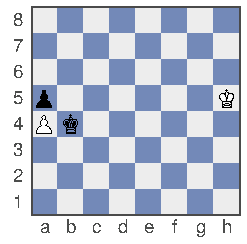
\includegraphics[width=\linewidth]{figures/trebuchet_2025.pdf}
\caption{\pos{W~Kh5~a4 / \mbox{B~Kb4~a5}}}
\label{fig:trebuchet_2025}
\end{subfigure}\hfill
\begin{subfigure}{0.32\columnwidth}
\centering
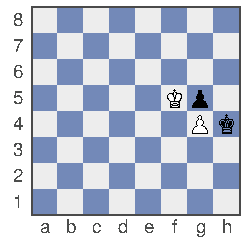
\includegraphics[width=\linewidth]{figures/trebuchet.pdf}
\caption{\pos{W~Kf5~g4 / \mbox{B~Kh4~g5}}}
\label{fig:trebuchet}
\end{subfigure}\hfill
\begin{subfigure}{0.32\columnwidth}
\centering
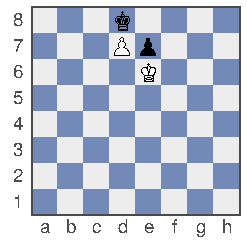
\includegraphics[width=\linewidth]{figures/kinggroup72.pdf}
\caption{\pos{W~Ke6~d7 / \mbox{B~Kd8~e7}}}
\label{fig:kinggroup72}
\end{subfigure}
\caption{King groups: (a) a tr\'ebuchet on the cylinder (files a and h adjacent) and (b) the tr\'ebuchet T
(ordinary board), both real mutual zugzwangs that count as $0$; (c) a king group from the 2025 study (cylinder;
Section~\ref{sec:sums}) that does not count as $0$: it draws with white to move, a zugzwang for black only.}
\label{fig:kings}
\end{figure}

\subsection{When Is the Frozen Tr\'ebuchet Exact?}\label{sec:kings-valid}

A \emph{king group} $Z$ is the two kings and some pawns on a block of files whose neighboring files, the
\emph{buffer}, hold no pawns; a \emph{decisive event} is a move in $Z$ or one creating a passed pawn.

\begin{theorem}[Validity of the convention; \lab{S}]\label{thm:validity}
Let a position consist of pawn components and a king group $Z$ with its buffer, and suppose that before the
first decisive event:
\begin{enumerate}
\item[(V1)] outside $Z$ the legal chess moves are exactly the model's pawn moves, with the same results (en
  passant included); none gives check, nobody is in check, and the side to move has a legal move (one in $Z$
  counts);
\item[(V2)] in chess, the side that gets a passed pawn wins, and a race is won as the race rule says;
\item[(V3)] in chess, every move in $Z$ loses (it is \emph{decisively punished}).
\end{enumerate}
Then the chess result, with either side to move, is the outcome of $W(X)$, the pawn game that ends at the first
passed pawn (Section~\ref{sec:sums-hss}), without draws, where $X$ is the position with $Z$ and its pawns deleted.
\end{theorem}

\begin{proof}[Proof sketch]
By (V3) neither side moves in $Z$ without losing, so until the first decisive event both play the pawn game;
by (V1) the side to move always has a legal move, a pawn move or a move in $Z$; the pawn game is finite, so some
decisive event occurs, and by (V2) and (V3) that event
decides the chess game as it decides $W(X)$.
\end{proof}

\begin{corollary}[\lab{S}]\label{cor:v4}
If also (V4) $X$ is hereditarily sum-safe (Definition~\ref{def:hss}) and satisfies condition (E) of
Theorem~\ref{thm:hss}, and $\BIG$ exceeds the number of moves either side can make, the chess result is
the outcome class of the components' $\pm\BIG$ value.
\end{corollary}

\begin{proof}
By Theorem~\ref{thm:validity} the chess result is the outcome of $W(X)$, and by Theorem~\ref{thm:hss} this is
the outcome of $S(X)$.
\end{proof}

Each condition can fail: a stalemate trap leaves the loser without a move (V1), a passed pawn does not win its
race (V2), a king walks over to the pawns or, in Fig.~\ref{fig:kinggroup72}, white's king moves go unpunished
(V3), and a $+\BIG$ cancels a $-\BIG$ (V4).

A local test for (V3) is the \emph{certificate of horizon $h$} of a move in $Z$: (i) with the pawns outside $Z$
removed, the punisher promotes within $h$ of its own moves after its reply, even if the defender may pass; (ii)
after the reply, with the defender to move and the punisher's king and all pawns in $Z$ removed, no defender
pawn in the context can promote within $h$ of its own moves (its pawns in $Z$ fall under (i)) (the \emph{counter-promotion condition}); (iii) the defender is never stalemated on the forcing
line. It works in the \emph{promotion game}, where the first promotion
wins.

\begin{theorem}[\lab{S}]\label{thm:cert}
In the promotion game, a move in $Z$ with a certificate of horizon $h$ is a loss for its mover, so the
promotion-game analogue of (V3) holds wherever every move in $Z$ has one; for chess, (V3) needs the further
check that a won promotion race is a won game. Clause (ii) cannot be weakened to $h-1$ moves.
\end{theorem}

In chess small margins fail. On the cylinder with seven files and six ranks, Kb4, Pe4 against Ka1, Pa2 with
white to move, the king move Kb4--c5 has a certificate of horizon~1, yet the chess result after it is a draw, and
Kc5--d5 in Kc5, Pe2 against Ka3, Pc4 on the same board has horizon~2, yet White wins \lab{C1}.

For (V2) a local test is known only if king moves also lose \lab{S}: a passed pawn then wins the promotion
game if, besides conditions on checks, stalemates and its own nearby pawns, its path is empty and every enemy
pawn, passed or not, needs a move more to promote. The model looks only at passed pawns: with Pc2, Pd4 against
Pd3 on the $8\times6$ cylinder, black to move, it credits white, yet d3$\times$c2 and c1=Q come first \lab{C1}.

\begin{proposition}[\lab{S}]\label{prop:horizon1}
On boards with at least six ranks, for $h=1$, the counter-promotion condition holds in every chess-legal
context without a passed pawn.
\end{proposition}

\begin{proof}
A pawn that can promote in one move stands on the rank before its last. With six or more ranks it got there by a
single step or a capture, so it cannot be taken en passant, and no enemy pawn can stand ahead of it: it is
already passed.
\end{proof}

\begin{conjecture}[\lab{Conj}]\label{conj:horizon2}
On a board with room for two files beyond the buffer, for every king group whose punishment needs $h\ge2$
moves, some context without a passed pawn leaves a move in the group unpunished.
\end{conjecture}

Real tr\'ebuchets seem to need $h\approx5$--$7$ \lab{Conj}, so we trust their zero only beside slow or locked components.

\subsection{Spare King Moves Are Loopy}

A king that can step back and forth without loss gives its side unlimited waiting moves, a loopy
game~\cite{WinningWays,Siegel2013}: $\textsf{on}=\game{\textsf{on}}{}$ if only white can wait,
$\textsf{off}=-\textsf{on}$ if only black can, and $\textsf{dud}$ if both can. Since $\textsf{on}$ exceeds every number, $\BIG$ included, the $\pm\BIG$ convention fails there, and a
decisive event must instead end the game.

\begin{theorem}[Outcomes with spare moves; \lab{S}]\label{thm:loopy}
Let the components form a short game in which every decisive event ends the game, let a side that can wait pass
at any time, and let every other move in $Z$ lose. If only white can wait, black wins exactly when it can force a decisive
event in its favor against a passing white, and white wins otherwise. If both can wait, a side wins exactly when
it can do so against a passing opponent, and otherwise the game is drawn.
\end{theorem}

\begin{proof}[Proof sketch]
If only white can wait, every play is finite, since black's moves are, so the game is determined, and black
wins exactly when some move of black's wins against every white reply, a pass included. If both can wait, a
winning side never needs to pass, so it wins exactly when it can force a decisive event against passes;
otherwise play can go on forever.
\end{proof}

Beside a spare king move, then, component values matter only through their forcing threats. The kings
alone are already loopy: in normal play (a stalemate loses), every quiet K+P against K placement on the boards
from $3\times4$ to $5\times5$, summed with sixteen test games, behaves as a decisive win, $\textsf{on}$,
$\textsf{off}$ or $\textsf{dud}$, or as none of these; none behaves as a number or an infinitesimal, and removing
the edges changes the class of $12.5$--$20.5\%$ of them \lab{C2}.

\subsection{How Often Does the Convention Fail?}\label{sec:kings-sweep}

We solved, with the kings played out, every component with at most two pawns a side beside a
tr\'ebuchet on boards with six ranks: on one file of the six-file cylinder and of the five-file ordinary board,
and on files d and e of the seven-file cylinder (queen promotions only, at most two). Of these, $500$ start without a race and have a determined result. Under the textbook test, $159$ of the $500$ get the wrong outcome \lab{C1}: $107$ through
the kings alone, $18$ through en passant and $34$ because a passed pawn does not win its race. $143$ of the
$159$ are on the seven-file cylinder. The e.p.-aware test repairs the $18$ e.p.\ failures, but the kings undo $13$ of these repairs. On the ordinary $8\times8$ board, in $94$ positions beside a tr\'ebuchet checked against the tablebase, the
convention says all $449$ king moves lose, yet $41$ draw and $7$ win \lab{C1}. The $34$ race failures have one cause: a blocked
enemy pawn steps level with its blocker and promotes first. Ending the game only at a passer that wins the
race by the square rule removes all $52$ convention failures and leaves $128$ mismatches, all from the
kings \lab{C1}. Over the $2{,}049$ decisive $8\times8$ positions beside a tr\'ebuchet whose real results we know,
the model agrees with chess in $92.5\%$; the count rule beats the mover and opponent rules ($83\%$)
\lab{C1}.

\section{Sums, Temperature and the Puzzles Revisited}\label{sec:sums}

Most endgames are sums of components. We recall two principles for playing them, apply them to three puzzles,
and ask when a sum names the same winner as the whole board.

\subsection{Two Principles}

\emph{Principle 1 (number avoidance).} In a sum of numbers and games that are not numbers, a player who can win
can do so without moving in a number~\cite{WinningWays,Siegel2013}.

\emph{Principle 2 (the hottest move).} Move in the component with the highest temperature
(Section~\ref{sec:notation}). For a switch $\game{x}{y}$ between numbers $x>y$, the temperature $(x-y)/2$ is
what each side gains by moving there first, and infinitesimals have temperature $0$. Principle~2 is a
heuristic, not a theorem, but it finds the winning move in every example below.

\subsection{The Puzzles Revisited}

\begin{figure}[!t]
\centering
\begin{subfigure}{0.32\columnwidth}\centering
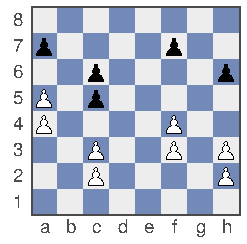
\includegraphics[width=\linewidth]{figures/puzzle71.pdf}
\caption{Puzzle 1}\label{fig:puzzle71}
\end{subfigure}\hfill
\begin{subfigure}{0.32\columnwidth}\centering
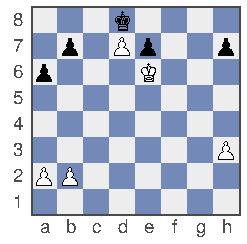
\includegraphics[width=\linewidth]{figures/puzzle72.pdf}
\caption{Puzzle 2}\label{fig:puzzle72}
\end{subfigure}\hfill
\begin{subfigure}{0.32\columnwidth}\centering
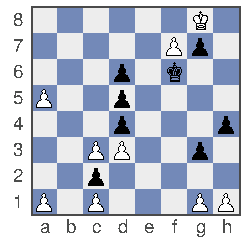
\includegraphics[width=\linewidth]{figures/puzzle73.pdf}
\caption{Puzzle 3}\label{fig:puzzle73}
\end{subfigure}
\caption{The three puzzles of~\cite{Study2025} (cylinder: files a and h adjacent); Table~\ref{tab:puzzles}
gives their exact values. (a)~White wins whoever moves first. (b)~The pawn part is an infinitesimal.
(c)~Puzzle~3 as first drawn: $+\BIG$ (not legal).}
\label{fig:puzzles}
\end{figure}


Fig.~\ref{fig:puzzles} shows three puzzles on the cylinder, and Table~\ref{tab:puzzles} compares the values
first claimed for them~\cite{Study2025} with the exact ones; the earlier walk-throughs pick the right
winners, but not always the right values.

\begin{table}[!t]
\centering
\caption{Puzzles of Fig.~\ref{fig:puzzles}: Claimed and Exact Values \lab{C2}}
\label{tab:puzzles}
\begin{tabular}{@{}lll@{}}
\toprule
Part & Claimed~\cite{Study2025} & Exact \\
\midrule
1: c-file & $\pm1$ & $\pm1$ \\
1: f-file & $\game{\game{2}{1}}{0}$ & the same (mean $3/4$) \\
1: files h, a & $1$ & $\game{+\BIG}{\star}$ (hot) \\
1: total & $1\pm1+\game{\game{2}{1}}{0}$ & white wins either way \\
2: pawns & $\pm1$ & infinitesimal, mean $0$ \\
2: kings & $0$ & not a zugzwang \\
3: files c, d & $1$ & $\tinyg{1}$ \\
3: total & $2$ & $+\BIG$ before any move \\
\bottomrule
\end{tabular}
\end{table}

\emph{Puzzle 1} (Fig.~\ref{fig:puzzle71}) has three components. The earlier values of the c-file, $\pm1$, and of
the f-file, $\game{\game{2}{1}}{0}$ with mean $3/4$, are right. Files h and a are not. White's a5--a6 still wins
outright, but black, moving first, plays h6$\times$a5 across the seam and leaves $\star$, not a loss, so this
part is $\game{+\BIG}{\star}$, hot, not the number $1$. The total is still a white win whoever moves first, but
play now starts in the h/a component, by far the hottest (Principle~2). White to move plays a5--a6 and wins.
Black to move does best to take on a5 at once, since every other move lets white force a passed pawn (after
h6--h5, for example, a4$\times$h5); white then plays c3--c4 in the next hottest component, and
$1+\star+\game{\game{2}{1}}{0}$ is a white win whoever moves next.

\emph{Puzzle 2} (Fig.~\ref{fig:puzzle72}) has one pawn component, on files h, a and b. The earlier walk-through
finds the right first moves, h3--h4 and a6--a5, and the right outcome, a first-player win. But the value is an
infinitesimal with mean $0$, not $\pm1$, so by Principle~2 it waits until every hot component is settled.
Its king group (Fig.~\ref{fig:kinggroup72}) is not a tr\'ebuchet either. With black to move, the d7 pawn covers
c8 and e8, so Kc7 is forced, and white takes e7 and promotes. With white to move, Kd5, Ke5 and Kf5 all draw:
black wins the d7 pawn, but the white king blockades the e-pawn. The group is a zugzwang for black only, on the
ordinary board \lab{C2} (our solver and the Lichess tablebase) and on the cylinder \lab{C1}, so the real result
of this ten-man position is open.

\emph{Puzzle 3} (Fig.~\ref{fig:puzzle73}) is illegal, with four white pawns on the first rank, and as drawn it
is decided at once, since the pawns on a5 and f7 are passed. On files c and d, white's best move, c3$\times$d4,
leaves $0$. Black's only move, d4$\times$c3, leaves $\game{0}{-1}$: white locks the files with d3--d4, while
black's d5--d4 keeps the spare move d6--d5. Thus $G=\ggame{0}{0\mid -1}=\tinyg{1}$, not $1$, and the legal copy
one rank up, \pos{W c2 c4 d4 / B c3 d5 d6 d7}, has the same value.

\subsection{When Is the Sum Model Right?}\label{sec:sums-hss}

In chess the first passed pawn ends the game; in a sum, a component with a passed pawn becomes $\pm\BIG$ and
play goes on elsewhere, so a $+\BIG$ can cancel a $-\BIG$. In $\game{\BIG}{0}+\game{0}{-\BIG}$ the first player
makes a passed pawn and wins the chess game, but the sum is $0$ for every $\BIG$, since the second player
answers in the other component \lab{P}. We write $S(X)$ for the sum model of a pawn position $X$ and $W(X)$ for
the whole-board game, which ends at the first passed pawn.

\begin{definition}[Hereditary sum safety]\label{def:hss}
A component carries a \emph{threat} for a side if a position reachable from it gives that side a passed pawn. A
position $X$ is \emph{hereditarily sum-safe} (HSS) if no position reachable from $X$ by moves of either side,
in any order, before the first passed pawn, $X$ included, has two components with threats for opposite sides.
\end{definition}

\begin{theorem}[Sum safety; \lab{AI}]\label{thm:hss}
Suppose that $X$ is HSS, that no position reachable from $X$ with two or more components has a usable en
passant right (condition (E)), and that $\BIG$ exceeds the number of moves either side can make. Then $S(X)$ and $W(X)$ have the same
outcome.
\end{theorem}

\begin{proof}[Proof sketch]
The models differ only after a passed pawn appears, say for white. By HSS no other component can then give black
one, so in the sum black runs out of moves before white's $+\BIG$ does. The full proof, by induction with (E),
is in the repository.
\end{proof}

In a random sample of $1{,}500$ positions, all $1{,}297$ HSS ones agree \lab{C1}, and with $\BIG=256$ the move
bound always holds on boards with eight ranks. HSS cannot be dropped (Proposition~\ref{prop:sumcounter});
without (E) the decomposition already fails in the pure pawn game (Proposition~\ref{prop:condE}).

\begin{proposition}[\lab{C2}]\label{prop:sumcounter}
A test of the top-level components alone is not enough: on $\cyl{8}$ with en passant off, $X=$\,\pos{W b2 d4 g3
h5 / B a7 c7 f7 g4} is a single component, spanning files f to d across the seam, so such a test passes it; yet
$S(X)$ is a black win whoever starts, while $W(X)$ is a first-player win.
\end{proposition}

Components with opposite threats appear only later in its tree, so $X$ is not HSS.

\begin{proposition}[\lab{C1}]\label{prop:condE}
In the pure pawn game, without the passed-pawn rule (play goes on until a side has no move), (E) cannot
be dropped: the sum can be wrong, even in outcome. On the ordinary board with six files and six ranks take
\pos{W a4 f4 / B b4 e5}, where black may take b4$\times$a3 en passant, since white has just played a2--a4. The
whole board is $\game{0}{-4,\,-3\pm2}$, a first-player win, while the sum of its two components is
$\game{-1\star}{-5\star}$, a black win: in the sum the en passant right survives moves in the other component. The two differ
with white to move, the case that arises inside larger sums; with black to move, as in the chess position,
both say black wins.
\end{proposition}

\emph{Two models.} Our CGT engine adds up components, as Elkies does~\cite{Elkies1996}; the independent
whole-board solver ends the game at the first passed pawn. Wherever the two disagree, in every case we tested,
our engine with splitting switched off matches the whole-board solver. The two models agree on every headline value: the $1/8$ and $\upsec\star$
positions of Section~\ref{sec:targets} in all nine settings (Section~\ref{sec:ep}), and the seven-pawn $\nim{2}$
of Section~\ref{sec:star2} in the default setting. Elsewhere they can differ, even in outcome: under the
opponent rule with the e.p.-aware test, \pos{W a3 b3 c2 e2 / B a6 c5 d5 e3} (the first five-file $\nim{2}$ of
Section~\ref{sec:star2-five}) is ${\Uparrow}$ as a sum but $\nim{2}$ on the whole board. Where they differ, we name the model we mean.

\section{The Atlas: What Only the Cylinder Can Do}\label{sec:atlas}

We computed two collections of positions with every pawn on ranks 2--7, at least one pawn per side and no
passed pawn. \emph{The atlas} holds every such position with at most five pawns on
$\cyl{3},\dots,\cyl{8}$ and $\flatb{3},\dots,\flatb{8}$, up to symmetry: $1{,}223{,}689$ positions
\lab{C1}. An independent minimax program confirms their textbook winners for all
$12{,}568$ rings and $4{,}000$ random ordinary components. \emph{The census} holds every such position
with at most six pawns on $\flatb{1},\dots,\flatb{4}$, up to translation and mirror image:
$231{,}071$ records standing for $459{,}443$ positions.

Under the textbook test, the atlas values free of $\BIG$ include just two nimbers: $\star$, and one
$\nim{2}$, the textbook candidate of Section~\ref{sec:star2}, which the e.p.-aware test removes. They also
include several ups, such as ${\Uparrow}\star$ on one file (Section~\ref{sec:basic-inf}), and fractions with
denominator at most $4$, of which $3/4$ and $-3/4$ occur only on $\cyl{3}$.

\begin{figure}[!t]
\centering
\begin{subfigure}[b]{0.36\columnwidth}\centering
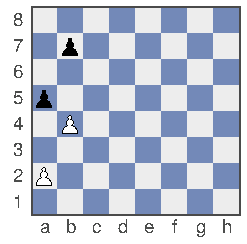
\includegraphics[height=1.05in]{figures/hot3.pdf}
\caption{}
\end{subfigure}\hfill
\begin{subfigure}[b]{0.18\columnwidth}\centering
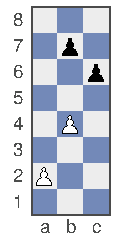
\includegraphics[height=1.05in]{figures/ring3_threequarters.pdf}
\caption{}
\end{subfigure}\hfill
\begin{subfigure}[b]{0.18\columnwidth}\centering
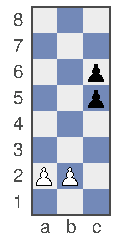
\includegraphics[height=1.05in]{figures/ring3_quarter.pdf}
\caption{}
\end{subfigure}\hfill
\begin{subfigure}[b]{0.22\columnwidth}\centering
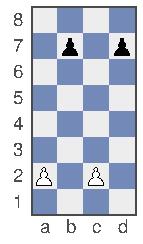
\includegraphics[height=1.05in]{figures/ring4.pdf}
\caption{}
\end{subfigure}
\caption{Atlas values. (a)~The hottest, $\pm3$ (ordinary board). (b)--(d)~Values that occur only on
cylinders (file a next to the last file) under the textbook test: (b)~$3/4$ and (c)~$1/4\pm1/4$ on
$\cyl{3}$, (d)~the $\nim{2}$ candidate's pawns on $\cyl{4}$, not a $\nim{2}$.}
\label{fig:hot3}
\end{figure}

\subsection{The Hottest Position}
Apart from $\pm\BIG$, the highest temperature in the atlas under the textbook test is $3$, reached by white
a2, b4 against black a5, b7 (Fig.~\ref{fig:hot3}(a)). Whoever moves first captures. If white does,
b4$\times$a5 leaves the b7-pawn stuck, since either step lets the a5-pawn through, and white three spare
moves ahead: $3$. If black does, a5$\times$b4 leaves $-3$. Thus $G=\game{3}{-3}=\pm3$ \lab{C1}.

\subsection{Cylinder-Only Values}
A value that occurs on a cylinder but on no ordinary board is \emph{cylinder-only}. By the cut lemma
(Theorem~\ref{thm:cut}) it comes from a ring, which on $n$ files needs $n$ pawns.

\begin{proposition}[\lab{C1}]\label{prop:cylonly}
Under the textbook test, $53$ atlas values free of $\BIG$ are cylinder-only: $40$ from $3$-file rings and
$13$ from $4$-file rings; the five-pawn rings on $\cyl{5}$ give none. No atlas value occurs only on ordinary boards.
\end{proposition}

On $\cyl{3}$, white a2, b4 against black b7, c6 is $3/4$ and white a2, b2 against black c5, c6 is
$1/4\pm1/4$, under both tests (Fig.~\ref{fig:hot3}(b), (c)). On $\cyl{4}$, the pawn list of the $\nim{2}$
candidate of Section~\ref{sec:star2}, white a2, c2 against black b7, d7, is a different game, since files a and
d are adjacent across the seam: $\game{3/2\pm1/2}{-3/2\pm1/2}$ under the textbook
test but $\game{2\pm1}{-2\pm1}$ under the e.p.-aware test, a value that also occurs on the ordinary board.

Nor are these values robust: the $3$-file ones depend on the race rule ($3/4$ becomes $0$ under the mover
rule), the $4$-file ones on the e.p.\ option. We compared all nine settings only for positions with at most
four pawns; among them no value is cylinder-only in all nine \lab{C1}.

\section{Elkies' Small Values}\label{sec:targets}

Elkies~\cite{Elkies1996} found fractions, ups and tinies in chess endgames on the ordinary board. We searched
the census (Section~\ref{sec:atlas}) for smaller values of these kinds: $1/8$, $1/16$ and $1/32$;
\emph{up-second} $\upsec=\game{0}{{\downarrow}\star}$, positive but smaller than ${\uparrow}$, and
$\upsec\star=\game{0,\star}{{\downarrow}}$; and the \emph{tinies} $\tinyg{x}=\ggame{0}{0\mid -x}$ (a number $x$).
Table~\ref{tab:targets} counts them under both passed-pawn tests; under the e.p.-aware test $1/32$
disappears.

\begin{table}[!t]
\caption{Elkies' Small Values in the Census}
\label{tab:targets}
\centering
\begin{tabular}{@{}llcc@{}}
\toprule
Value & Form & Textbook & E.p.-aware \\
\midrule
$1/8$ & $\game{0}{1/4}$ & $13$ & $9$ \\
$1/16$ & $\game{0}{1/8}$ & $3$ & $2$ \\
$1/32$ & $\game{0}{1/16}$ & $1$ & $0$ \\
$\upsec$ & $\game{0}{{\downarrow}\star}$ & $5$ & $2$ \\
$\upsec\star$ & $\game{0,\star}{{\downarrow}}$ & $10$ & $10$ \\
$\tinyg{1}$ & $\ggame{0}{0\mid -1}$ & $13$ & $16$ \\
$\tinyg{x}$, $x\notin\mathbb{Z}$ & $\ggame{0}{0\mid -x}$ & $0$ & $0$ \\
\bottomrule
\end{tabular}

\smallskip
\parbox{\columnwidth}{\footnotesize Positions of each exact value in the census (count rule). Textbook
column: an independent C solver confirmed each identity (position minus target $=0$) \lab{C2}. E.p.-aware
column: \lab{C1}.}
\end{table}

\begin{figure}[!t]
\centering
\begin{subfigure}[b]{0.32\columnwidth}\centering
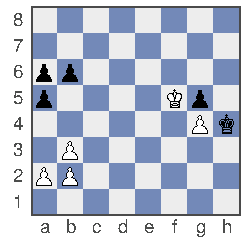
\includegraphics[width=\linewidth]{figures/eighth.pdf}
\caption{}
\end{subfigure}\hfill
\begin{subfigure}[b]{0.32\columnwidth}\centering
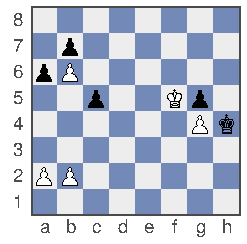
\includegraphics[width=\linewidth]{figures/upsecstar.pdf}
\caption{}
\end{subfigure}\hfill
\begin{subfigure}[b]{0.32\columnwidth}\centering
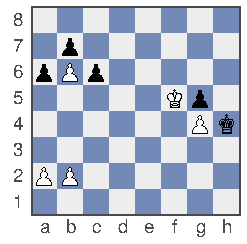
\includegraphics[width=\linewidth]{figures/tiny1.pdf}
\caption{}
\end{subfigure}
\caption{Elkies' small values beside T (Fig.~\ref{fig:trebuchet}), each a 10-man position with a legal pawn
history (ordinary board). (a)~$1/8$: \pos{W a2 b2 b3 / B a5 a6 b6}. (b)~$\upsec\star$: \pos{W a2 b2 b6 / B a6 b7 c5}.
(c)~$\tinyg{1}$: \pos{W a2 b2 b6 / B a6 b7 c6}.}
\label{fig:eighth}
\end{figure}

\subsection{A Reachable Eighth}

\begin{theorem}[\lab{C2}]\label{thm:eighth}
In the pawn model, white a2, b2, b3 against black a5, a6, b6 has value exactly $1/8$ in all nine settings
(Section~\ref{sec:ep}) and for every assignment of outcomes to its race positions.
\end{theorem}

To see why, look at Fig.~\ref{fig:eighth}(a). If white moves first, a2--a4 locks the a-file and leaves the
zero game. The quieter a2--a3 reaches only $\star$, from which black can return to $0$, so it is reversible.
The move b3--b4 is bad, since black's reply leaves $-3$. If black moves first, b6--b5 leaves $1/4$, and
a5--a4 is bad. Thus $G=\game{0}{1/4}=1/8$.

This pawn structure can arise in a game: from the starting position, c2$\times$b3, a7--a5, b7$\times$a6 and
c7$\times$b6 produce it. Its mirror image, white a2, a3, b2 against black a6, b5, b6, cannot, since its
a3-pawn could only have come from a2 or b2, and both are still on their starting squares. The independent
checks were run on the mirror, which has the same value by symmetry: a C solver confirms both parts of the
theorem, and a third, separately written solver confirms the value in all nine settings. Section~\ref{sec:real} tests the $1/8$ with real kings.

\subsection{Up-Second Star and Tiny~1}
White a2, b2, b6 against black a6, b7, c5 (Fig.~\ref{fig:eighth}(b)) is $\upsec\star$ in all nine settings
\lab{C2}. If white moves first, a2--a4 leaves $0$ and a2--a3 leaves $\star$. If black moves first, a6--a5
leaves ${\downarrow}$. Thus $G=\game{0,\star}{{\downarrow}}=\upsec\star$.

Now move the black c-pawn back to c6 (Fig.~\ref{fig:eighth}(c)). If white moves first, a2--a3 leaves $0$.
If black moves first, a6--a5 leaves $-1/2\pm1/2=\game{0}{-1}$, and c6--c5, which reaches the $\upsec\star$
position, is dominated, since $\game{0}{-1}\le\upsec\star$. Thus $G=\ggame{0}{0\mid -1}=\tinyg{1}$ under
every race rule with en passant on (textbook test \lab{C2}, e.p.-aware test \lab{C1}); with e.p.\ off it is
${\uparrow}$. Unlike the Tiny~1 of Section~\ref{sec:basic-inf}, it needs no seam. Both pawn structures
arise from the starting position by c2$\times$b3, b3--b4--b5--b6, a7--a6 and c7--c5 (c7--c6 for Tiny~1).

\subsection{Two Textbook Values That Fail}
Under the textbook test the census also has a $1/8$ at white a2, b2, d2 against black a5, c4, d7 and an
$\upsec$ at white a3, c5, d4 against black a7, b7, d7. The e.p.-aware test makes them $-3/2\pm3/2$ and
$\game{3/4}{{\downarrow}\star}$. Both rested on counting as passed a pawn that
could still be taken en passant. This is why we state Theorem~\ref{thm:eighth} and the $\upsec\star$ above for
all nine settings.

\section{The \texorpdfstring{$\nim{2}$}{*2} Question}\label{sec:star2}

The $\nim{2}$ question of Section~\ref{sec:intro} asks whether a king-and-pawn position on a board with eight
ranks can have this value. We show that the only $\nim{2}$ in the census under the textbook test
comes from that test, that none exists with six pawns or fewer in the default setting, and that $\nim{2}$
appears with seven.

\subsection{The Textbook Candidate}

\begin{figure}[!t]
\centering
\begin{subfigure}{0.32\columnwidth}\centering
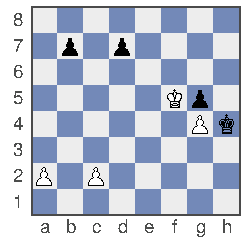
\includegraphics[width=\linewidth]{figures/star2_textbook.pdf}
\caption{Candidate}\label{fig:star2_textbook}
\end{subfigure}\hfill
\begin{subfigure}{0.32\columnwidth}\centering
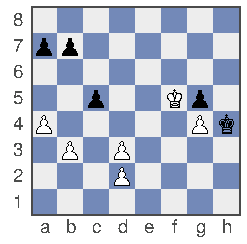
\includegraphics[width=\linewidth]{figures/star2_seven_a.pdf}
\caption{Position A}\label{fig:star2_seven_a}
\end{subfigure}\hfill
\begin{subfigure}{0.32\columnwidth}\centering
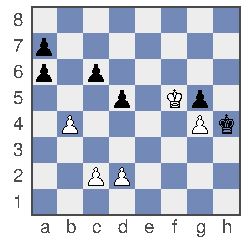
\includegraphics[width=\linewidth]{figures/star2_seven_b.pdf}
\caption{Position B}\label{fig:star2_seven_b}
\end{subfigure}
\caption{Positions of the $\nim{2}$ question beside T (Fig.~\ref{fig:trebuchet}; ordinary board). (a)~Candidate:
$\nim{2}$ under the textbook test, $\game{2\pm1}{-2\pm1}$ under the e.p.-aware test. (b)~Position A and
(c)~position B: $\nim{2}$ in the default setting (count rule, e.p.-aware test).}
\label{fig:star2}
\end{figure}

Fig.~\ref{fig:star2_textbook} shows the candidate \pos{W a2 c2 / B b7 d7} on files a--d. Under the count rule
with the textbook test, it is the only $\nim{k}$ with $k\ge2$ in the census of Section~\ref{sec:atlas}. If white
moves first, a2--a4 leaves $\star$ and c2--c4 leaves $0$; a2--a3 and c2--c3 are worse. The position is symmetric
(turn the board around and swap the colors), so black's d7--d5 leaves $\star$ and b7--b5 leaves $0$. Thus
$G=\game{0,\star}{0,\star}=\nim{2}$.

The weak point is black's plan b7--b5 and b5--b4. After b5--b4 the a-pawn is in the situation of
Fig.~\ref{fig:ep_test}: the textbook test scores a2--a4 as a passed pawn, $+\BIG$, but in chess black takes
b4$\times$a3 en passant. Under the e.p.-aware test, \pos{W a2 c2 / B b4 d7} is worth $-3$, a black win, so
b7--b5 is worth $-2\pm1$ and, by symmetry, c2--c4 is worth $2\pm1$. The other moves, among them a2--a4 and
d7--d5, which still lead to $\star$, are dominated or reversible. Hence
\[
G=\game{2\pm1}{-2\pm1},
\]
a hot game with mean $0$ and temperature $2$ \lab{C2}.

\subsection{No \texorpdfstring{$\nim{2}$}{*2} With Six Pawns or Fewer}

\begin{theorem}[Census; \lab{C2}]\label{thm:census}
In the census of Section~\ref{sec:atlas}, in the default setting, no position has value $\nim{k}$ with
$k\ge2$; the census has $6{,}724$ zeros and $4{,}042$ stars.
\end{theorem}

Our CGT engine and an independent C solver, which tests whether $G+\nim{k}$ is a second-player win, agree on
every record, and the independent whole-board solver finds no $\nim{k}$ with $2\le k\le 292$ among
$793{,}299$ labeled placements on widths 1--4 (every placement on each width, without reduction by symmetry or
translation). Every position in scope has birthday (Section~\ref{sec:notation}) at most $292$, so no
larger nimber can occur. Under the textbook test the census has $6{,}470$ zeros, $3{,}891$ stars and the
candidate; the e.p.-aware test removes that $\nim{2}$. In non-default settings a few other census
positions are $\nim{2}$; Section~\ref{sec:real-cand} tests one of them in real chess.

\subsection{\texorpdfstring{$\nim{2}$}{*2} With Seven Pawns}

\begin{theorem}[$\nim{2}$ with seven pawns; \lab{C2}]\label{thm:star2seven}
In the default setting, position~A, \pos{W a4 b3 d2 d3 / B a7 b7 c5}, and position~B,
\pos{W b4 c2 d2 / B a6 a7 c6 d5}, on files a--d of the ordinary board, have value $\nim{2}$, and both fit beside T, with the capture
histories c2$\times$d3 (A) and b7$\times$a6 (B). Neither is $\nim{2}$ with e.p.\ off or under the opponent rule.
\end{theorem}

In position A (Fig.~\ref{fig:star2_seven_a}), if white moves first, a4--a5 leaves $0$. The move d3--d4 attacks
c5; every black reply except c5$\times$d4 loses at once, and after c5$\times$d4 white continues b3--b4 to
$\star$, so the reversible move d3--d4 counts as a move to $\star$. White's third move, b3--b4, loses to
c5$\times$b4. If black moves first, a7--a5 leaves $0$ and b7--b6 leaves $\star$. Black's other moves are
reversible: after a7--a6 and b7--b5 white has replies worth $2$ and $3$, both at least $\nim{2}$; and c5--c4
lets d3$\times$c4 free white's d2 pawn for $+\BIG$. Thus
$G=\game{0,\star}{0,\star}=\nim{2}$.

In position B (Fig.~\ref{fig:star2_seven_b}), if white moves first, d2--d4 leaves $0$ and c2--c3 leaves
$\star$. The moves d2--d3 and c2--c4 are reversible, since black's replies reach $-2$ and $-3$, and b4--b5
loses to a6$\times$b5. If black moves first, d5--d4 leaves $0$, and a6--a5 attacks b4: every white reply except
b4$\times$a5 loses at once, and after b4$\times$a5 black continues c6--c5 to $\star$, so a6--a5 counts as a move
to $\star$. Black's third move, c6--c5, loses to b4$\times$c5. Thus $G=\nim{2}$ again.

\begin{table}[!t]
\centering
\caption{Values of the Three $\nim{2}$ Positions in the Model Settings}
\label{tab:star2_settings}
\footnotesize
\setlength{\tabcolsep}{4pt}
\begin{tabular}{@{}lccc@{}}
\toprule
Race rule, passed-pawn test & Candidate & A & B\\
\midrule
count, e.p.-aware & $\game{2\pm1}{-2\pm1}$ & $\nim{2}$ & $\nim{2}$\\
mover, e.p.-aware & $\game{2\pm1}{-2\pm1}$ & $\nim{2}$ & $\nim{2}$\\
count or mover, textbook & $\nim{2}$ & $\nim{2}$ & $\nim{2}$\\
count or mover, e.p.\ off & $\nim{2}$ & not $\nim{2}$ & not $\nim{2}$\\
opponent, any e.p.\ option & $0$ & not $\nim{2}$ & not $\nim{2}$\\
\bottomrule
\end{tabular}
\end{table}

In Table~\ref{tab:star2_settings} (e.p.\ on unless stated) every entry is \lab{C2}; for A and B, our CGT
engine, the census scanner that found them and the independent whole-board solver agree on each. The candidate
needs the textbook test but survives e.p.\ off; A and B need en passant but not the textbook test.

\subsection{Counts and Five Files}\label{sec:star2-five}

On ordinary boards of width at most four, in the default setting, two $\nim{2}$ positions have seven pawns and
four have eight. One exhaustive scan of $5{,}503{,}282$ root positions gives these counts, so their
completeness is \lab{C1}; our engine re-checked every position it reported \lab{C2}. With
Theorem~\ref{thm:census}, seven is the least number of pawns in a $\nim{2}$ on these boards \lab{C2}.

On five files a scan of all $14{,}680{,}983$ eight-pawn positions finds $21$ of value $\nim{2}$ in the default
setting \lab{C1}, each using all five files. As whole-board games all $21$ are $\nim{2}$: the whole-board solver
and our engine with splitting switched off agree \lab{C2}. As sums of components (Section~\ref{sec:sums-hss})
$15$ keep the value; the other six change only through the splitting. Three of the
$21$ come from the $14$ eight-pawn $\nim{2}$ rings on $\cyl{5}$ \lab{C1} by opening them onto files a--e:
\begin{itemize}
\item \pos{W a3 b3 c2 e2 / B a6 c5 d5 e3},
\item \pos{W a4 b3 c2 d2 / B a7 b6 c7 e4},
\item \pos{W a6 b4 c4 e3 / B a7 c7 d6 e6},
\end{itemize}
and these are $\nim{2}$ in both models. We call the first \emph{the five-file $\nim{2}$}. No $\nim{3}$ or higher nimber occurs in the default setting in any scope we searched
\lab{C1}.

By Theorem~\ref{thm:cut}, a pawn position on $\cyl{n}$ with an empty file is one on $\flatb{n-1}$, so these
scans also cover such positions on $\cyl{3}$ to $\cyl{5}$. A ring has no empty file. One scan of the rings on
$\cyl{5}$ to $\cyl{8}$ with at most eight pawns finds $\nim{2}$ in the default setting only in the $14$
eight-pawn rings on $\cyl{5}$ \lab{C1}. Narrower cylinders need fewer pawns. On $\cyl{3}$ the only ring
$\nim{2}$ with six pawns in the default setting is \pos{W a2 a3 b2 / B b7 c6 c7}, and on $\cyl{4}$ the first
are \pos{W a4 b2 c2 / B b6 c5 d6 d7} and its color-reversed twin, with seven; our engine confirms both values
\lab{C2}. No ring with fewer pawns is a $\nim{2}$ on either cylinder (the atlas up to five pawns, and a C scan
of every six- and seven-pawn split) \lab{C1}. On $\cyl{6}$ the first rings have nine pawns: a scan of every
nine-pawn ring finds six \lab{C1}, among them \pos{W a4 c4 d2 e2 / B b6 b7 d6 e5 f6}; both programs confirm
three, and the other three are their color-reversed twins \lab{C2}. So the first ring
$\nim{2}$ on $\cyl{n}$ has $n+3$ pawns for $n=3,\dots,6$. The $\cyl{3}$ ring needs en passant (with e.p.\ off its value is $0$), and it is a $\nim{2}$ with
one pawn fewer than any ordinary board of width at most four allows. Rings also carry $\nim{3}$, though not in
the default setting: with e.p.\ off, the eight-pawn ring \pos{W a5 b3 c2 d2 / B a7 b5 c6 d4} on $\cyl{4}$ is
$\nim{3}$ under the opponent rule, and the ten-pawn ring \pos{W a2 a3 b2 b3 c3 / B a6 a7 b6 b7 c6} on $\cyl{3}$
under the count rule \lab{C2}.

In the model, then, the $\nim{2}$ question has a positive answer on the ordinary $8\times8$ board: four files
and seven pawns beside T suffice, while Elkies' higher nimbers need larger boards~\cite{Elkies2002}. Whether real
chess agrees is the subject of Section~\ref{sec:real}.

\section{From the Model to Real Chess}\label{sec:real}

To test a model value, we keep its tree of pawn moves and replace only the leaves by real results: from the
Lichess Syzygy tablebase~\cite{LichessTB} up to seven men, and beyond from tablebase-backed search and our
king-and-pawn solver (Section~\ref{sec:kings}).

\begin{definition}[Real-chess oracle value]\label{def:oracle}
Let $X$ be a pawn component on the ordinary board beside T (Fig.~\ref{fig:trebuchet}). An \emph{end position}
of its model tree is a position where a line of play first reaches a passed pawn; its two \emph{sides} are
white to move and black to move. Replace each end position by $+\BIG$ if white wins it in real chess with either
side to move, by $-\BIG$ if black does, by $\game{+\BIG}{-\BIG}$ if the side to move wins, and by $0$ if the
side to move loses. If a side is drawn, the \emph{draw treatment} counts that draw as a win for black, as a win
for white, or as worth $0$; in the last case the end position is $\game{\BIG r_W}{\BIG r_B}$, where
$r_W,r_B\in\{-1,0,1\}$ are white's results with white and with black to move. All these games lie between $-2\BIG$ and $2\BIG$. The canonical value of the resulting tree is the \emph{oracle value} $O(X)$.
\end{definition}

\begin{lemma}[Sandwich; \lab{P}]\label{lem:sandwich}
Replace every end position not known to be $\pm\BIG$ by $-2\BIG$, or by $+2\BIG$, and let $O^-$ and $O^+$ be the
resulting values. Then $O^-\le O(X)\le O^+$ whatever the draw treatment and the unknown results; if $O^-=O^+$, then
$O(X)$ is certified.
\end{lemma}
\begin{proof}
Every leaf lies between $-2\BIG$ and $2\BIG$, and raising an option never lowers a
game~\cite{Siegel2013}; induct from the leaves.
\end{proof}

\subsection{The Textbook Candidate in Real Chess}\label{sec:real-cand}

We build the tree under either passed-pawn test, the \emph{textbook tree} or the \emph{e.p.-aware tree}.

\begin{theorem}[Candidate in real chess; \lab{C1}]\label{thm:oracle-cand}
For the candidate \pos{W a2 c2 / B b7 d7} beside T (Fig.~\ref{fig:star2_textbook}):
\begin{enumerate}
\item[(a)] In real chess the side to move wins; only 1\ldots~b5 wins for black, 1.~c4 wins for white, and every
  king move loses \lab{C2}.
\item[(b)] In the e.p.-aware tree, under every draw treatment, $O$ has left stop $\ge1$ and right stop $\le-1$, so
  $O$ is neither $0$ nor $\nim{2}$.
\item[(c)] If draws count as wins for black, $O=\game{2\pm1}{-2\pm1}$ in both trees.
\end{enumerate}
\end{theorem}

Real chess thus agrees with $\nim{2}$ on the outcome and on every winning first move resolved so far
(1.~a4 is still open), but not on the value: in the e.p.-aware tree, which matches chess, $O$ is always hot. In
the textbook tree $\nim{2}$ is ruled out only when draws count as wins for one side, as in (c), so the
candidate's $\nim{2}$ depends on the textbook test.

A second candidate, \pos{W a3 b3 c2 / B b5 b7 c6} ($10$ men with T), is $\nim{2}$ under the opponent
rule with en passant on (Section~\ref{sec:star2}); its oracle value is positive under every draw treatment
\lab{C1}. The other non-default $\nim{2}$ positions are open.

\subsection{Towards a Real-Chess \texorpdfstring{$1/8$}{1/8}}\label{sec:real-eighth}

The $1/8$ position of Section~\ref{sec:targets} (Fig.~\ref{fig:eighth}(a)) has $10$ men. Its e.p.-aware tree
has $302$ end-position sides with at most seven men, and the tablebase resolves them all. In $290$ of them
only one side has a passed pawn: $283$ agree with the model, $5$ disagree and $2$ are draws; the other $12$ are
races. A search for the larger end positions that decide the value finds five with eight men and three with
nine. Four of the eight-man ones are resolved: seven of their sides agree with the model, and black to move in
\pos{W a3 a5 / B b4 b5} is a black win against it. A second search allows for that result and leaves one
eight-man position and the three of nine men to decide the value. Our king-and-pawn solver (queen promotions
only) shows that all four agree with the model on both sides; the hardest, black to move in
\pos{W b2 b5 / B a5 b4}, needed two promoted queens in the search, $6.1\times10^{10}$ states in $15$ hours.

\begin{proposition}[A real-chess $1/8$; \lab{C1}]\label{prop:eighth-real}
For the $1/8$ position, with queen promotions only in our solver, $O=1/8$, whatever the end positions that are
still open do.
\end{proposition}

This $1/8$ assumes the frozen kings of the tree (Section~\ref{sec:kings}), and a rerun with underpromotions
would make it a full-chess certificate. The same method applies to $\upsec\star$ and $\tinyg{1}$: their lower bounds already equal the
target values, with $11$ and $13$ end positions of $8$ to $10$ men still open \lab{C1}. Positions A and B have $11$ men beside
T, and the five-file $\nim{2}$ \pos{W a3 b3 c2 e2 / B a6 c5 d5 e3}, which sits legally
beside T, has $12$, with only file f free of pawns between them. Their oracle values are open. For A and B a
search finds end positions that decide the value; the five and seven of them with $8$ men agree with the model
(queen promotions only) \lab{C1}, but those with $9$ to $11$ men are unsolved, so the $\nim{2}$ of
Theorem~\ref{thm:star2seven} is so far a model value.

\section{Mating Without Corners: Tablebases}\label{sec:tb}

We now bring in the pieces and ask a classical question: without corners, which material can still force
mate? We computed the tablebases of eight pawnless endings, king and one or two pieces against the bare
king, on the ordinary board, on the cylinder and on the torus, where ranks 1 and 8 are joined as well. Chess
on these boards is an old variant~\cite{Pritchard}. Prose sources say that king and rook cannot force mate
on the cylinder, nor king and queen on the torus~\cite{WikiCylinder,HGMCylinder}; we confirm the torus claim,
but the rook mates from 2.80\% of cylinder positions. We found no earlier tablebase for them.

\emph{Rules.} Pieces move as in Section~\ref{sec:rules} and wrap round each glued edge. There is no castling
and no fifty-move rule, and stalemate and bare kings are draws. A position is legal when the kings are not
adjacent, across the seams included, and the side not to move is not in check. Both dimensions of the board
are even, so the coloring of the squares survives the gluing.

\emph{Verification.} Two retrograde solvers, written independently from these rules, agree on every position
of all 24 tables, about 607 million values with either side to move \lab{C2}. On the ordinary board both
reproduce the known longest mates.

\begin{table}[!t]
\centering
\caption{Pawnless Endings Against the Bare King on the Ordinary Board, Cylinder and Torus: Share Won With
White to Move and Longest Mate \lab{C2}}
\label{tab:tb}
\footnotesize
\setlength{\tabcolsep}{4.5pt}
\begin{tabular}{@{}lrrrrrr@{}}
\toprule
& \multicolumn{2}{c}{Ordinary} & \multicolumn{2}{c}{Cylinder} & \multicolumn{2}{c}{Torus} \\
\cmidrule(lr){2-3}\cmidrule(lr){4-5}\cmidrule(l){6-7}
Material & Won (\%) & Mate & Won (\%) & Mate & Won (\%) & Mate \\
\midrule
KQK  & 100    & 10 & 100    & 10 & 0      & --- \\
KRK  & 100    & 16 & 2.80   & 3  & 0      & --- \\
KBBK & 99.98  & 19 & 100    & 14 & 0      & --- \\
KBNK & 99.51  & 33 & 0.0245 & 2  & 0      & --- \\
KNNK & 0.0107 & 1  & 0.0077 & 1  & 0      & --- \\
KRBK & 100    & 16 & 99.74  & 13 & 0.0218 & 1   \\
KRRK & 100    & 7  & 100    & 8  & 100    & 7   \\
KQRK & 100    & 6  & 100    & 5  & 100    & 5   \\
\bottomrule
\end{tabular}

\smallskip
\parbox{\columnwidth}{\footnotesize Mate: longest forced mate in moves; ---: no position is won. KBBK has
the bishops on opposite colors.}
\end{table}

On the cylinder the queen ignores the seam: KQK wins every position, as quickly as on the ordinary board.
KRK, KBNK and KNNK do not, and on the torus not even the queen can force mate
(Table~\ref{tab:tb}).

\emph{KRK and KBNK rarely force mate on the cylinder.} The first and eighth ranks are still edges, but now
closed loops with no corner. The rook wins only 2.80\% of the positions, all from mating nets already
in place, such as Ka3, Rb2 against Ka1: 1.~Rb3 Kh1 2.~Rg3 Ka1 3.~Rg1\#. The rook covers h1 and the
white king h2, the two flight squares across the seam. Bishop and knight win even more rarely: their mate
needs a corner of the bishop's color, and the cylinder has none.

\emph{Bishops on opposite colors win every position on the cylinder}, and faster than on the ordinary board,
although the bishop pair is said not to mate there~\cite{HGMCylinder}.
Here the seam helps the attacker: every diagonal winds round from the first rank to the eighth. The longest
line ends in Ke6, Be1, Bf1 against Ke8: the bishop on f1 checks along f1--h3--a4--e8, across the seam, and
the bishop on e1 covers d8 and f8.

\emph{On the torus, of the eight endings, only KRRK and KQRK force mate}, and they win from every position. KRBK wins only where
a mate in one is already set up, and the bishop pair has mating positions that no legal white move can
produce.

\emph{Twisted boards.} KRK wins everywhere on the M\"obius strip (files a and h joined, ranks reversed), but
only $0.66\%$ on the Klein bottle, which also joins ranks 1 and 8 \lab{C2}.

\subsection{King and Pawn Against King}\label{sec:kpk}

We solved every legal KPK position on the $8\times8$ ordinary board and cylinder twice, with our
king-and-pawn solver of Section~\ref{sec:kings} (all four promotions) and with a separately written KPK
solver (queen promotion only). They agree on all 326,640 cylinder positions and differ on exactly 6
ordinary-board positions, where only a rook promotion wins, such as Ka4, Pb7 against
Ka6 \lab{C2}. Table~\ref{tab:kpk} gives the counts; the cylinder has fewer legal positions, since the kings
may not touch across the seam and, with white to move, the black king may not stand where the white
pawn attacks across the seam.

\begin{table}[!t]
\centering
\caption{King and Pawn Against King: Legal Positions and White Wins on the $8\times8$ Ordinary Board and
Cylinder \lab{C2}}
\label{tab:kpk}
\footnotesize
\begin{tabular}{@{}lrrrr@{}}
\toprule
& \multicolumn{2}{c}{White to move} & \multicolumn{2}{c}{Black to move} \\
\cmidrule(lr){2-3}\cmidrule(l){4-5}
Board & Legal & White wins & Legal & White wins \\
\midrule
Ordinary & 163,328 & 124,960 & 168,024 & 97,604 \\
Cylinder & 160,656 & 126,736 & 165,984 & 92,760 \\
\bottomrule
\end{tabular}
\end{table}

\begin{figure}[!t]
\centering
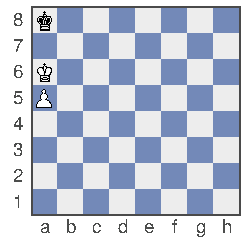
\includegraphics[width=0.26\columnwidth]{figures/kpk_rookpawn.pdf}
\caption{Ka6, Pa5 against Ka8, with either side to move: a white win on the cylinder (files a and h adjacent),
a draw on the ordinary board.}
\label{fig:kpk_rookpawn}
\end{figure}

Fig.~\ref{fig:kpk_rookpawn} shows the classic rook-pawn draw: on the ordinary board the black king cannot be
driven out of the corner without stalemate. On the cylinder we may shift every man four files to the right,
which gives Ke6, Pe5 against Ke8, the textbook win whoever is to move. Back on the a-file, with black to move,
play goes 1\ldots~Kb8 2.~Kh7 Kb7 3.~a6+, and the pawn promotes under the king, which guards a7 and a8 from h7.

Of the positions legal on both boards, 16,538 ordinary-board draws become cylinder wins. The seam also
helps the defender, since a king on the h-file now stands beside an a-pawn: 15,930 ordinary-board wins
become cylinder draws. Zugzwang, the engine of the tr\'ebuchet, is more common on the cylinder: 216
reciprocal zugzwangs (white to move draws, black to move loses) against 160 on the ordinary board
\lab{C2}.

\begin{table}[!t]
\centering
\caption{King and Pawn Against King on $\cyl{n}$: White-to-Move Wins and Reciprocal Zugzwangs \lab{C2}}
\label{tab:oddw}
\footnotesize
\begin{tabular}{@{}lrrr@{}}
\toprule
$n$ & Legal, white to move & White wins (\%) & Reciprocal zugzwangs \\
\midrule
3 & 5,706   & 53.00 & 0   \\
4 & 16,008  & 65.87 & 208 \\
5 & 34,350  & 73.92 & 95  \\
6 & 63,036  & 76.55 & 132 \\
7 & 104,370 & 77.49 & 175 \\
8 & 160,656 & 78.89 & 216 \\
\bottomrule
\end{tabular}
\end{table}

\emph{Other widths.} Table~\ref{tab:oddw} covers $\cyl{n}$ for $n=3,\dots,8$, where two independently
written solvers agree \lab{C2}; one widened solver gives 79.41\% and 79.94\% for $n=9,10$ \lab{C1}. Odd
and even widths behave alike: the win rate rises with $n$, and from $n=4$ on the share of reciprocal zugzwangs falls,
from 1.30\% to 0.13\% at $n=8$. The tr\'ebuchet of Fig.~\ref{fig:trebuchet_2025} is a mutual zugzwang (the side to
move loses either way) for $4\le n\le8$ \lab{C2} and $n=9$ \lab{C1}, and illegal on $\cyl{3}$. Ka3, Pa2 against
Ka5, a draw on the ordinary board, is a reciprocal zugzwang for $4\le n\le8$ \lab{C2} and $n=9,10$ \lab{C1}. On $\cyl{3}$, Ka1, Pa7 against Ka3
wins at once: a8=Q checks along the a-file, which covers a4, and the wrapped diagonals and the white king cover
the other flight squares \lab{C2}.

\emph{A pawn each.} With all promotions but at most one new piece, our solver decides 89\% of the 14.6 million
KPKP placements on the cylinder (14.9 million on the ordinary board) and 83\% on the ordinary board \lab{C1}
(placements with an e.p.\ right pending are not enumerated). Of the positions decided on both,
10\% change result, three quarters of them to a draw, and 576 pairs of reciprocal zugzwangs exist only on the
cylinder, 20 of them mutual: in Ka3, Ph2 against Kg2, Ph3 whoever moves loses, since Ka3 reaches the
locked pawns across the seam; a second solver agrees on a sample \lab{C2}.

\section{Dawson's Chess on the Cylinder}\label{sec:dawson}

On a cylinder every file is alike, and the first move opens the ring of files into an ordinary strip. The
earlier study~\cite{Study2025} used this idea on Dawson's chess but stated the game incorrectly; here
we restate it and redo the analysis.

\begin{figure}[!t]
\centering
\begin{subfigure}{0.48\columnwidth}
\centering
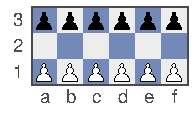
\includegraphics[scale=0.8]{figures/dawson_strip.pdf}
\caption{}
\label{fig:dawson_strip}
\end{subfigure}\hfill
\begin{subfigure}{0.48\columnwidth}
\centering
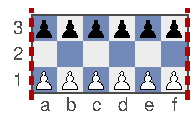
\includegraphics[scale=0.8]{figures/dawson_ring.pdf}
\caption{}
\label{fig:dawson_ring}
\end{subfigure}
\caption{Starting position of Dawson's chess on six files. (a) $3\times6$ ordinary board. (b) $3\times6$
cylinder: files a and f are adjacent; dashed edges are glued.}
\label{fig:dawson_boards}
\end{figure}

\begin{figure*}[!t]
\centering
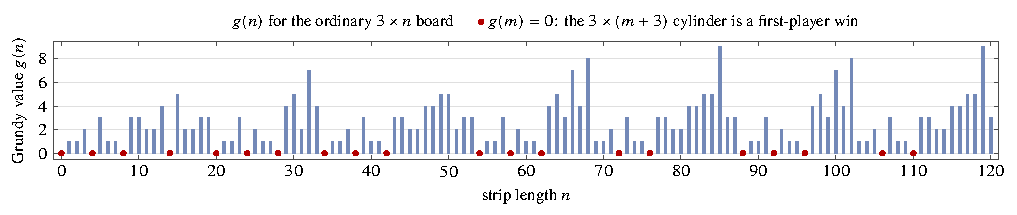
\includegraphics[width=\textwidth]{figures/dawson_grundy.pdf}
\caption{Grundy values $g(n)$ of Dawson's chess on the $3\times n$ ordinary board (octal game
$\mathbf{0.137}$), $n\le120$. Dots mark $g(m)=0$: the $3\times m$ board is a second-player win and the
$3\times(m+3)$ cylinder a first-player win (Theorem~\ref{thm:ring}).}
\label{fig:dawson_grundy}
\end{figure*}

\emph{Rules.} Dawson's chess~\cite{Dawson1935} is played on a $3\times n$ board
(Fig.~\ref{fig:dawson_boards}) with white pawns on rank~1, black pawns on rank~3 and rank~2 empty. Pawns move
and capture as in chess, captures are compulsory, and no pawn can double-step or promote. The last player to
move wins; in the mis\`ere form that Dawson posed, the last player loses.

Let us see what one move does. Call a file \emph{untouched} if both its pawns stand on their starting
squares. Suppose white plays c1--c2 with the b- and d-files untouched. The pawn on c2 attacks b3 and d3, so
black must capture, say b3$\times$c2. That pawn attacks b1 and d1, so white must recapture, say
d1$\times$c2, and then come d3$\times$c2 and b1$\times$c2. This leaves black to move, with the b- and
d-files empty and the c-file blocked for good, since a pawn enters a file only by capturing. At the end of a
row the push takes three plies and empties its one neighbor; a push with no untouched neighbor is
blocked.

Each such sequence is forced and touches only the pushed file and its neighbors. Counting a whole sequence as
one move, strips separated by empty files never interact, and both players have the same sequences, so this
game of sequences is impartial. A strip of $n$ untouched files is therefore the octal game $\mathbf{0.137}$~\cite{GuySmith1956,WinningWays},
in which a move removes a file and its untouched neighbors. Its Grundy values are $g(0)=0$, $g(1)=1$ and,
for $n\ge2$,
\begin{equation}\label{eq:dawson}
g(n)=\operatorname{mex}\bigl(\{g(n-2)\}\cup\{g(a)\oplus g(b) : a+b=n-3\}\bigr),
\end{equation}
where $a,b\ge0$, $\oplus$ is the nim-sum and mex is the least non-negative integer not in the set. The first
player wins the ordinary $3\times n$ board exactly when $g(n)\ne0$. The values from~\eqref{eq:dawson}
have period 34 with last exception $n=51$~\cite{GuySmith1956}, which two programs reproduce for $n\le300$
\lab{C2}.

\emph{What was wrong.} In~\cite{Study2025} a pawn could be removed from a single row only when
both its neighbors were empty, so a full row of two or more pawns has no move. Its recurrence lacks the
end-file term $g(n-2)$ of~\eqref{eq:dawson} and the value $g(1)=1$, agrees with $g$ at only 31 of the 301 values
$n\le300$, and gives the wrong cylinder outcome for 56 of them \lab{C2}. The first is $n=4$, a predicted
first-player win: white's push and four captures leave one untouched file, black pushes that pawn, it is
blocked, and white has no move.

\begin{theorem}[Ring rule; \lab{P}, machine-checked for $n\le22$]\label{thm:ring}
On the full $3\times n$ cylinder, $n\ge3$, every first move with its forced captures leaves one strip of
$n-3$ untouched files, with the opponent to move. Hence the cylinder has Grundy value
$\operatorname{mex}\{g(n-3)\}$, and the first player wins if and only if $g(n-3)=0$, that is, for
$n=3,7,11,17,23,27,31,37,41,45,57,\dots$
\end{theorem}

\begin{proof}
Every file of a full ring has two distinct untouched neighbors, so every push starts the five-ply sequence
above. The other $n-3$ files, bounded by empty files that never change, form an ordinary strip. By
rotation all first moves are alike, and the cylinder has one option.
\end{proof}

The ring formula of~\cite{Study2025} and its remark that the ring's value is always 0 or 1 are
right once the correct $g$ is used (Fig.~\ref{fig:dawson_grundy}).

\emph{Mis\`ere play.} A forced sequence has odd length and ends with the player who began it, so the
ring rule carries over: the first player wins the mis\`ere cylinder exactly when the strip of $n-3$ files is
a mis\`ere P-position. Our implementation of the Plambeck--Siegel algorithm~\cite{PlambeckSiegel2008}
reproduces their partial quotient for strips of at most 32 files (order 638, 109 P-positions) and agrees
with exhaustive search on 7.4 million positions \lab{C2}; our computation of the next quotient, for longer strips, did not finish.

\emph{A warning about sums.} As a partizan game on its own, the ordinary $3\times5$ board is $\star$,
although $g(5)=3$. The outcome agrees, but only $g$ adds up: a sum of such values would let a player reply
elsewhere while a capture is pending.

% Table of the Appendix. It is input before Section XII so that the table* float lands on the page that
% holds the Appendix text, before the Acknowledgment and the reference list.
\begin{table*}[!t]
\centering
\caption{Main Positions with Kings}
\label{tab:positions}
\footnotesize
\setlength{\tabcolsep}{4pt}
\begin{tabular}{@{}>{\raggedright\arraybackslash}p{0.29\textwidth}p{0.05\textwidth}%
  >{\raggedright\arraybackslash}p{0.255\textwidth}>{\raggedright\arraybackslash}p{0.335\textwidth}@{}}
\toprule
Role and value & Board & Men (white / black) & FEN \\
\midrule
\multicolumn{4}{@{}l}{\emph{Kings and puzzles}} \\
Tr\'ebuchet across the seam & $\cyl{8}$ & \pos{W Kh5 a4 / B Kb4 a5} &
\fen{8/8/8/p6K/Pk6/8/8/8} \\
Tr\'ebuchet T & $\flatb{8}$ & \pos{W Kf5 g4 / B Kh4 g5} & \fen{8/8/8/5Kp1/6Pk/8/8/8} \\
Puzzle~2 king group: white to move draws & $\cyl{8}$ & \pos{W Ke6 d7 / B Kd8 e7} &
\fen{3k4/3Pp3/4K3/8/8/8/8/8} \\
Puzzle~2: pawns infinitesimal, mean $0$ & $\cyl{8}$ & \pos{W Ke6 a2 b2 d7 h3 / B Kd8 a6 b7 e7 h7} &
\fen{3k4/1p1Pp2p/p3K3/8/8/7P/PP6/8} \\
\midrule
\multicolumn{4}{@{}l}{\emph{Elkies' small values}} \\
$1/8$, in all nine settings & $\flatb{8}$+T & \pos{W a2 b2 b3 / B a5 a6 b6} &
\fen{8/8/pp6/p4Kp1/6Pk/1P6/PP6/8} \\
$\upsec\star$, in all nine settings & $\flatb{8}$+T & \pos{W a2 b2 b6 / B a6 b7 c5} &
\fen{8/1p6/pP6/2p2Kp1/6Pk/8/PP6/8} \\
Tiny~1 & $\flatb{8}$+T & \pos{W a2 b2 b6 / B a6 b7 c6} & \fen{8/1p6/pPp5/5Kp1/6Pk/8/PP6/8} \\
Textbook $1/8$, now $-3/2\pm3/2$ & $\flatb{8}$+T & \pos{W a2 b2 d2 / B a5 c4 d7} &
\fen{8/3p4/8/p4Kp1/2p3Pk/8/PP1P4/8} \\
Textbook $\upsec$, now $\game{3/4}{{\downarrow}\star}$ & $\flatb{8}$+T & \pos{W a3 c5 d4 / B a7 b7 d7} &
\fen{8/pp1p4/8/2P2Kp1/3P2Pk/P7/8/8} \\
\midrule
\multicolumn{4}{@{}l}{\emph{The $\nim{2}$ question}} \\
Candidate: $\game{2\pm1}{-2\pm1}$; textbook $\nim{2}$ & $\flatb{8}$+T &
\pos{W a2 c2 / B b7 d7} & \fen{8/1p1p4/8/5Kp1/6Pk/8/P1P5/8} \\
Second candidate: opponent-rule $\nim{2}$, oracle $>0$ & $\flatb{8}$+T &
\pos{W a3 b3 c2 / B b5 b7 c6} & \fen{8/1p6/2p5/1p3Kp1/6Pk/PP6/2P5/8} \\
Position A: $\nim{2}$ & $\flatb{8}$+T & \pos{W a4 b3 d2 d3 / B a7 b7 c5} &
\fen{8/pp6/8/2p2Kp1/P5Pk/1P1P4/3P4/8} \\
Position B: $\nim{2}$ & $\flatb{8}$+T & \pos{W b4 c2 d2 / B a6 a7 c6 d5} &
\fen{8/p7/p1p5/3p1Kp1/1P4Pk/8/2PP4/8} \\
Five-file $\nim{2}$ & $\flatb{8}$+T & \pos{W a3 b3 c2 e2 / B a6 c5 d5 e3} &
\fen{8/8/p7/2pp1Kp1/6Pk/PP2p3/2P1P3/8} \\
\midrule
\multicolumn{4}{@{}l}{\emph{Real chess}} \\
Last $1/8$ end position: white wins (queens only) & $\flatb{8}$+T &
\pos{W b2 b5 / B a5 b4} & \fen{8/8/8/pP3Kp1/1p4Pk/8/1P6/8} \\
$1/8$ end position against the model: black to move wins & $\flatb{8}$+T &
\pos{W a3 a5 / B b4 b5} & \fen{8/8/8/Pp3Kp1/1p4Pk/P7/8/8} \\
KPK rook pawn: cylinder win, ordinary draw & $\cyl{8}$ &
\pos{W Ka6 a5 / B Ka8} & \fen{k7/8/K7/P7/8/8/8/8} \\
\bottomrule
\end{tabular}
\end{table*}

\section{Engines and Learning}\label{sec:engines}

CGT suggests which endgames may trouble an engine: an infinitesimal such as ${\uparrow}$ is a fight over one
spare tempo and a nimber such as $\star$ a fight over parity; neither shows in the material, so a static
evaluation can miss them until the search sees the fight's end.

\subsection{A CGT Test Suite}

We built $233$ legal positions on the ordinary $8\times8$ board with at most seven men, each labeled by its CGT class
(Table~\ref{tab:sf}). In $181$ of them the Lichess tablebase~\cite{LichessTB} confirms the winning moves that
CGT predicts; in the other $52$ the model and the tablebase disagree, so we score the engines against the
tablebase.

\subsection{Stockfish and Lc0}

We ran Stockfish~19~\cite{Stockfish} on one thread with a $64$~MB hash and no tablebases. It solves all $233$
positions at $10^5$ nodes, and $232$ already at $10^3$ \lab{C1}. The classes separate at a small fixed depth
(Table~\ref{tab:sf}). At depth~1 the engine reads hot positions, numbers and switches correctly
$73$--$81\%$ of the time, but infinitesimals only $30\%$ ($26\%$ at depth~2) and nimbers $53\%$
\lab{C1}, consistent with tempo and parity fights, though nimbers and the class \emph{other} are not clearly
separated at this sample size. Both classes reach $100\%$ by depth~8.
With one engine and a small sample, this is a pilot result.

\begin{table}[!t]
\centering
\caption{Stockfish~19 at Fixed Depth: Evaluations (\%) Matching the Tablebase, by CGT Class, Without the
Seven Decided ($\pm\BIG$) Positions}
\label{tab:sf}
\footnotesize
\begin{tabular}{@{}lrrrrrrr@{}}
\toprule
 & & \multicolumn{6}{c}{Search depth} \\
\cmidrule(l){3-8}
CGT class & $n$ & 1 & 2 & 4 & 6 & 8 & 12 \\
\midrule
hot ($\pm\BIG$ switch) & 68 & 81 & 78 & 91 & 97 & 99 & 100 \\
number & 57 & 79 & 81 & 84 & 93 & 95 & 98 \\
switch & 37 & 73 & 78 & 89 & 100 & 100 & 100 \\
other & 20 & 60 & 50 & 75 & 95 & 100 & 100 \\
nimber & 17 & 53 & 65 & 88 & 100 & 100 & 100 \\
infinitesimal & 27 & 30 & 26 & 59 & 85 & 100 & 100 \\
\bottomrule
\end{tabular}

\smallskip
\parbox{\columnwidth}{\footnotesize Infinitesimal: ups and downs, with or without $\star$. Other: values free of
$\BIG$ that fall in none of the other classes, such as tinies and games $\game{a\pm x}{b\pm y}$.}
\end{table}

Lc0~v0.32.1~\cite{Lc0}, with its bundled network, is perfect at all four budgets, $10^3$ to $10^6$ nodes,
all $17$ draws included \lab{C1}, so at practical budgets the suite is too easy for both engines.

\subsection{ChessSums}

Beyond seven men no tablebase applies, but CGT still values sums exactly. We built ChessSums, a set of
$26{,}000$ pawn-endgame sums whose components come from a library of $418$ with $37$ distinct values; every
component has the same value in all nine settings (Section~\ref{sec:ep}). Whole-board alpha--beta confirms every outcome
except five that hit its time limit \lab{C1}, and an independent minimax confirms $4{,}887$ of them
\lab{C2}. Alpha--beta, blind to the split,
needs about $4$--$9$ times as many nodes per added component \lab{C1}, while adding the CGT values costs
almost nothing.

\subsection{Engines on Sums}

We placed each sum on the ordinary $8\times8$ board beside T (Fig.~\ref{fig:trebuchet}) or a shifted copy that our
king-and-pawn solver confirms is a mutual zugzwang, giving legal positions with $15$--$20$ men. On $200$ of
them, Stockfish~19 picks a winning move only $26.5$--$28.0\%$ of the time from $10^3$ to $10^6$ nodes, and Lc0
$32.5$--$33.5\%$ at $10^3$ and $10^4$ nodes \lab{C1} ($34$--$36\%$ and $42$--$43\%$ without the $45$
second-player wins, which have no winning move). More nodes barely help, both engines worsen as components are
added, and the errors do not single out nimbers or infinitesimals. These numbers measure agreement with the
frozen-king model (not always exact; Section~\ref{sec:kings-sweep}), not real-chess errors.

\subsection{Learning Dawson's Chess}

In normal-play Dawson's chess the first player wins exactly when the strips' Grundy values have a nonzero
nim-sum~\cite{GuySmith1956,WinningWays}. An LSTM value network in PyTorch~\cite{PyTorch}, trained on total lengths up to
$30$, scores $0.82$ on lengths $31$--$80$, against $0.79$ for the majority guess \lab{C1}; the rule scores $1.0$,
and linear probes on the strip embedding do no better than the majority guess.

% \codeavail is defined in main.tex (named build: the repository URL; review build: anonymized).
% The fallback below only keeps this file compiling if main.tex does not define it.
\providecommand{\codeavail}{available at \expandafter\url\expandafter{\repourl}}

\section{Verification and Reproducibility}\label{sec:verify}

\emph{Cross-checks.} Our CGT engine agrees with a separate brute-force sum solver on $55{,}195$ positions $G$
(at most two pawns a side, $3$--$5$ files), for three race rules and $15$ reference games $X$: all
$4{,}967{,}550$ outcomes of $G+X$ match under the textbook test, e.p.\ on and off, and all $2{,}483{,}775$
under the e.p.-aware test. A whole-board minimax confirms its outcomes on $1{,}070$ single components. Our
legal-move generator matches Lichess on all $160$ test positions, covering en passant, promotions, pins, checks,
mates and stalemates. Each section states its other cross-checks.

\emph{Code availability.} The code and data are \codeavail. Our CGT engine and most tools are in
Python~3 (standard library only). The fast solvers (the king-and-pawn solver, the census scanner, the tablebase
generators) are in C. Real-chess checks use the Lichess Syzygy tablebase API. The engine
experiments use Stockfish~19 and Lc0. The learning baselines use PyTorch.

\section{Conclusion and Open Problems}\label{sec:conclusion}

Elkies' sum model holds up on a board without edges once the passed-pawn test respects en passant and the
frozen kings are checked. In the model, $\nim{2}$ appears with seven pawns and single-component $\nim{3}$ with nine
on ordinary boards and ten on the seven-file cylinder; with queen promotions and frozen kings the $1/8$ position
has oracle value exactly $1/8$. Six problems are open.

\begin{enumerate}
\item \emph{A certified $1/8$.} With queen promotions and frozen kings the oracle value is exactly $1/8$. Do
  the decisive end positions keep their results with all four promotions (Section~\ref{sec:real-eighth})?
\item \emph{The seven-pawn $\nim{2}$ in real chess.} The 8-man end positions deciding A and B agree with the
  model; those with 9 to 11 men are unsolved
  (Section~\ref{sec:real-eighth}).
\item \emph{Higher nimbers.} The least number of pawns in a ring $\nim{2}$ on $\cyl{n}$ is $n+3$ for $3\le n\le7$,
  ten for $7\le n\le10$ \lab{C2} and $n$ for every $n\ge10$ as a whole-board game \lab{S}. For $\nim{3}$ it is $n+2$ on $\cyl{10}$, $n+1$ on $\cyl{11}$ and at
  most $n+1$ up to $\cyl{59}$ \lab{C1}: can it be $n$? Are the wall
  families $\nim{2}$ as sums for all $n$? Is there a $\nim{4}$ on eight ranks?
\item \emph{When is a tr\'ebuchet zero?} Theorem~\ref{thm:cert} settles the promotion game, not chess: find a
  local test for chess, or settle Conjecture~\ref{conj:horizon2}; real tr\'ebuchets seem to have $h\approx5$--$7$ \lab{Conj}.
\item \emph{Endgames without edges.} With at most one new piece, $11\%$ of KPKP positions on the cylinder
  stay undecided, and KPPK comes next. Pawn play across the twisted seam of the M\"obius strip
  (Section~\ref{sec:tb}), where a pawn reverses direction, remains open.
\item \emph{Mis\`ere Dawson's chess.} Dawson asked about mis\`ere play \cite{Dawson1935}: is the mis\`ere
  quotient \cite{PlambeckSiegel2008} of Dawson's chess infinite? By the ring rule (Theorem~\ref{thm:ring}), an
  answer for strips also answers the cylinder.
\end{enumerate}


% The last page is short; keep its left column from being stretched to full height.
\raggedbottom
\appendix[Positions]
\label{app:positions}

Table~\ref{tab:positions} gives the FEN of each main position with kings. A men list gives the white men, then
the black men; K marks a king. On ``$\flatb{8}$+T'' the position stands on the ordinary
$8\times8$ board beside T (Fig.~\ref{fig:trebuchet}), and its FEN includes T. FENs give the piece placement
only; white is to move unless stated, and values are in the default setting (Section~\ref{sec:ep}). Pawn-only
positions are given by their pawn lists.


\section*{Acknowledgment}
The author thanks
\ifdefined\anonbuild\else
Prof.~T.~Morley for mentoring the 2025 study on which this work builds, and
\fi
the maintainers of the Lichess tablebase, Stockfish and Lc0 for making their tools freely available. AI
systems were used throughout this work, under the author's direction, and the author is responsible for the
content. Claude (Opus 5.5, Anthropic), run in Claude Code, wrote most of the software, ran the searches,
drafted the proofs and the figures, and drafted and revised the text of every section from
\ifdefined\anonbuild the 2025 study~\cite{Study2025}\else the author's 2025 study\fi{} and the project notes. Codex (OpenAI) wrote the independent whole-board solver and the census scanner
that found the seven-pawn positions. Nemotron 3 Ultra (NVIDIA) and MiniMax M3.1 Flash (MiniMax), run through
the Kilo and OpenCode tools, re-derived and repaired proofs and recomputed the reported king-and-pawn numbers.
Further models, chosen automatically by the Kilo, OpenCode and OmniRoute routers and not recorded by name,
carried out delegated checks and ran the engine experiments on sums and the Dawson learning experiment of
Section~\ref{sec:engines}. Statements labeled \lab{AI} have been checked only by these systems.


% (the odd-width table of Section X moved the references onto page 14)
% balance the last page's two columns of references
\ifdefined\anonbuild\IEEEtriggeratref{11}\else\IEEEtriggeratref{9}\fi
\bibliographystyle{IEEEtran}
\bibliography{refs}

\end{document}
